% !TeX spellcheck = en_GB
\chapter{Basics of category theory}
\label{ch:cats}

	Category theory takes a fairly general view of mathematical concepts. Instead of concentrating on details, it is the patterns and structures that are brought into focus here. The advantage of this approach is that methods that have proven helpful in one area of mathematics can be transferred to other areas, thus providing new (and possibly easier) proof techniques in these areas. The concept of categories was introduced by Samuel Eilenberg and Saunders Mac Lane in 1945 during their study of algebraic topology, while attempting to understand the processes that preserve mathematical structures \cite{Eilenberg1945}. A detailed treatment of the topic can be found in \cite{MacLane1998} and \cite{Borceux1994}, and more introductory texts are \cite{Leinster2009} and \cite{Awodey2010}. A more physics-oriented explanation of categories can be found in \cite{Baez2010} and \cite{Beer2018}, for example.

	In this thesis, we want to employ category theory to describe complex quantum systems, which is why we restrict ourselves to the basic definitions of category theory here. The systems of interest are \emph{anyons}, which are modelled by a specific type of category, namely Unitary Modular Tensor Categories (UMTCs). These come with the additional structure of a tensor category which allows us to describe composite systems and, moreover, the interaction of particles. Furthermore, they provide a graphical calculus that allows for a simple way of calculating properties of the system. We also introduce another specific type of categories, so-called trivalent categories, which describe some specific examples of anyon models in the next chapter. Although they cannot be used to generally treat anyons, it is worth to study these categories since their graphical calculus is extraordinarily simple. This makes trivalent categories an excellent source of simple examples for constructions that heavily rely on the graphical calculus.
	
	Although we limit ourselves to the basics of category theory here, we cannot avoid presenting a list of definitions, since learning a new mathematical concept is much like learning a new language: first, you need to learn a lot of vocabulary! 



\section{Basic definitions}

	
	\begin{defn}[Category]
		\label{def:cat}
		 A category\index{category} $\C$ consists of:
		 	\begin{itemize}
		 		\item a collection\footnote{We use the term \emph{collection} to indicate that this is not necessarily a set, but is, in general, too large to be a set. Think, for example, of the collection of all sets, which is not a set itself. This avoids running into Russel's paradox.} $\Obj(\C)$ of objects,
		 		\item for each pair of objects $X,Y\in\Obj(\C)$, a collection $\Hom_\C(X,Y)$\footnote{The notation ``Hom'' is of historical origin and stands for homomorphism, which appeared in one of the earliest examples of a category.} of morphisms\index{morphism} (or maps) from $X$ to $Y$,
		 		\item for each $X,Y,Z\in\Obj(\C)$, a function called composition:
		 				\begin{align}
			 				\Hom_\C(Y,Z)\times\Hom_\C(X,Y)&\to\Hom_\C(X,Z)\\
			 				(g,f)&\mapsto g\circ f,
		 				\end{align}
		 		\item for every object $X\in\Obj(\C)$, an element $\id_X\in\Hom_\C(X,X)$ called the identity on $X$.
		 	\end{itemize}
	 	These satisfy the following properties:
	 		\begin{enumerate}
	 			\item associativity: for each $f\in\Hom_\C(W,X)$, $g\in\Hom_\C(X,Y)$, and $h\in\Hom_\C(Y,Z)$ it holds that
	 					\begin{equation}
		 					(h\circ g)\circ f=h\circ(g\circ f),
	 					\end{equation} 
	 			\item identity laws: for every morphism $f\in\Hom_\C(X,Y)$, we have $f\circ\id_X=f=\id_Y\circ f$.
	 		\end{enumerate}
	\end{defn}

	\begin{rem} For convenience and/or clarity, we sometimes switch between different notations throughout this thesis:
		\begin{enumerate}
			\item We often write $X\in\C$ instead of $X\in\Obj(\C)$.
			\item We often write a morphism $f\in\Hom_\C(X,Y)$ as $f:X\to Y$ or depict it as
					\begin{figure}[h!]
					\begin{tikzpicture}
						\node (X) at (0,0) {$X$};
						\node (Y) at (1.5,0) {$Y$};
						\draw[->] (X) to node [above] {$f$} (Y);
					\end{tikzpicture}.
					\end{figure}
			\item We write $\Hom(X,Y)$ instead of $\Hom_\C(X,Y)$ whenever the category the morphisms live in is clear from the context.
		\end{enumerate}
	\end{rem}

	\begin{rem}
		If a morphism $f\in\Hom_\C(X,Y)$, we call $X$ the domain\index{domain} and $Y$ the codomain\index{codomain} of $f$. Every morphism in a category has a definite domain and a definite codomain.
	\end{rem}

	\begin{rem}
		Throughout this thesis, we will often use the terminology that a diagram commutes. This has the following meaning: Whenever there are two paths from an object $X$ to another object $Y$, the map from $X$ to $Y$ that is obtained by composing the maps along one path equals the map obtained by composing maps along the other path. For example, consider the diagram
		\begin{figure}[H]
			\begin{center}
				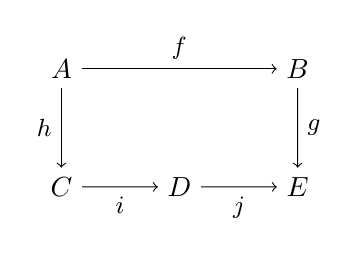
\begin{tikzpicture}[scale=1.5]
				\node (A) at (0,0) {$A$};
				\node (B) at (2,0) {$B$};
				\node (C) at (0,-1) {$C$};
				\node (D) at (1,-1) {$D$};
				\node (E) at (2,-1) {$E$};
				\draw[->] (A) to node [above] {\small $f$} (B);
				\draw[->] (B) to node [right] {\small $g$} (E);
				\draw[->] (A) to node [left] {\small $h$} (C);
				\draw[->] (C) to node [below] {\small $i$} (D);
				\draw[->] (D) to node [below] {\small $j$} (E);
				\end{tikzpicture}
			\end{center}
		\end{figure}
		\noindent
		This diagram is said to commute if $g\circ f=j\circ i\circ h$.
	\end{rem}

	\begin{defn}[Isomorphism]
		A morphism $f:X\to Y$ in a category $\C$ is an isomorphism\index{isomorphism} if it has an inverse, i.e., there exists a morphism $g:Y\to X$ such that $g\circ f=\id_X$ and $f\circ g=\id_Y$.
	\end{defn}
	This definition of an isomorphism is an example of the abstract way in which notions or concepts can be defined in the language of category theory. It has the advantage that, unlike other common definitions of isomorphisms, it does not use any additional structures than those given by the definition of the category. For example, an isomorphism of sets is usually defined as a bijective function, a definition that makes use of the \textit{elements} of the objects. 
	
	To illustrate the abstract definition, we have a look at some examples that include familiar mathematical objects such as sets and groups:
	
	\begin{exmp}[Category of Sets]
		\label{ex:sets}
		In the category of sets\index{Sets@$\mathbf{Sets}$}, denoted \textbf{Sets}, the objects are all possible sets. This implies that the collection of all objects of \textbf{Sets} itself is \emph{not} a set, but a class. The collection of morphisms from a set $X$ to a set $Y$, $\Hom(X,Y)$, consists of all maps $f:X\to Y$. Composition of morphisms then simply corresponds to the composition of maps. The identity morphism $\id_X:X\to X$ exists for every $X\in\Obj(\mathbf{Sets})$ and is given by the map $\mathbb{I}(a)=a$ for all $a\in X$.
	\end{exmp}

	\begin{exmp}[Group]
		\label{ex:grp}
		A group\index{group} $G$ can be described as a category $\mathcal{G}$ with a single object $\star$ and where all morphisms are isomorphisms. Here, $\Obj(\mathcal{G})=\{\star\}$ and there is only one collection of morphisms, namely $\Hom(\star,\star)$ which is given by the elements $g$ of the group $G$:
			\begin{equation}
				\Hom(\star,\star)=\{g|g\in G\}.
			\end{equation}
		Composition corresponds to the group operation (for example, multiplication) and the identity morphism is given by the unit object of the group. Since in a group every element has a unique inverse, every morphism in $\mathcal{G}$ is an isomorphism. This example illustrates a key guiding principle in category theory, namely, capturing the interesting structure within a category by the morphism sets $\Hom(X,Y)$ rather than in terms of complicated object classes.
	\end{exmp}


	Within a category, we are usually interested in connections, or maps, between objects. We can ask the same question about categories themselves, i.e., if there is a sensible notion of a map between categories. The answer to this question is yes, and the mathematical objects that describe these maps are called \emph{functors}\index{functor}:

	\begin{defn}[Functor]
		Let $\C$ and $\mathcal{D}$ be categories. A functor $F:\C\to\mathcal{D}$ between these categories consists of
			\begin{itemize}
				\item a function that assigns objects in $\C$ to objects in $\mathcal{D}$:
						\begin{align}
							\Obj(\C)&\to\Obj(\mathcal{D})\\
							X&\mapsto F(X),
						\end{align}
				\item for each $X,Y\in\C$, a function that maps morphisms in $\C$ to morphisms in $\mathcal{D}$:
						\begin{align}
							\Hom_C(X,Y)&\to\Hom_\mathcal{D}(F(X),F(Y))\\
							f&\mapsto F(f),
						\end{align}
			\end{itemize}
		which satisfy the following axioms: 
			\begin{enumerate}
				\item $F(g\circ f)=F(g)\circ F(f)$ for all composable morphisms $f,g$,
				\item $F(\id_X)=\id_{F(X)}$ for all $X\in\C$.
			\end{enumerate}
	\end{defn}

	\noindent
	Functors preserve the structure of a category: They preserve domains and codomains, identities, and composition. Hence, a functor $F:\C\to\mathcal{D}$ transforms a diagram in $\C$ into a---probably distorted---diagram in $\mathcal{D}$:
	\begin{figure}[H]
		\begin{center}
			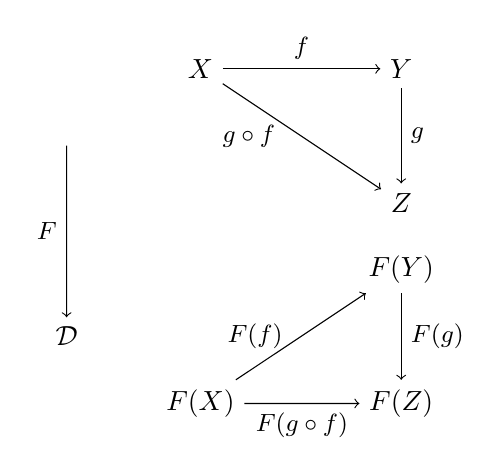
\begin{tikzpicture}[scale=0.85]
				\node (A) at (0,0) {$X$};
				\node (B) at (3,0) {$Y$};
				\node (D) at (3,-2) {$Z$};
				\draw[->] (A) to node [above] {\small $f$} (B);
				\draw[->] (B) to node [right] {\small $g$} (D);
				\draw[->] (A) to node [left] {\small $g\circ f\ \ $} (D);
				\node (B) at (3,-3) {$F(Y)$};
				\node (C) at (0,-5) {$F(X)$};
				\node (D) at (3,-5) {$F(Z)$};
				\draw[->] (B) to node [right] {\small $F(g)$} (D);
				\draw[->] (C) to node [left] {\small $F(f)\ $} (B);
				\draw[->] (C) to node [below] {\small $F(g\circ f)$} (D);
				\node (C1) at (-2,-1) {$\C$};
				\node (C2) at (-2,-4) {$\mathcal{D}$};
				\draw[->] (C1) to node [left] {\small $F$} (C2);
			\end{tikzpicture}
		\end{center}
	\end{figure}

	\begin{defn}[Natural transformation]
		Let $\C$ and $\mathcal{D}$ be categories and $F:\C\to\mathcal{D}$ and $G:\C\to\mathcal{D}$ be functors between them. A natural transformation\index{natural transformation} $\alpha:F\to G$ is a family of morphisms
			\begin{equation}
				\left(F(X)\xrightarrow{\alpha_X}G(X)\right)_{X\in\Obj(\C)}
			\end{equation}
		in $\mathcal{D}$, such that for every morphism $f:X\to X'$ in $\mathcal{C}$, the diagram
			\begin{figure}[H]
				\begin{center}
					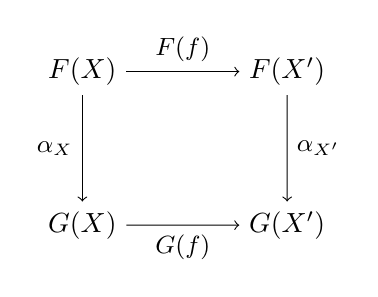
\begin{tikzpicture}[scale=1.3]
					\node (A) at (0,0) {$F(X)$};
					\node (B) at (2,0) {$F(X')$};
					\node (C) at (0,-1.5) {$G(X)$};
					\node (D) at (2,-1.5) {$G(X')$};
					\draw[->] (A) to node [above] {\small $F(f)$} (B);
					\draw[->] (B) to node [right] {\small $\alpha_{X'}$} (D);
					\draw[->] (A) to node [left] {\small $\alpha_X$} (C);
					\draw[->] (C) to node [below] {\small $G(f)$} (D);
					\end{tikzpicture}
				\end{center}
			\end{figure}
		\noindent
		commutes. The maps $\alpha_X$ are called the components of $\alpha$.
	\end{defn}

	In the same way that functors can be seen as maps between categories, i.e., as morphisms in the category of categories, natural transformations can be seen as maps between functors. There is indeed a notion of composition of natural transformations: Given two natural transformations $\alpha:F\to G$ and $\beta:G\to H$, with $F,G,H:\C \to\mathcal{D}$, there is a composite natural transformation $\beta\circ \alpha:F\to H$ which is defined by 
		\begin{equation}
			(\beta\circ \alpha)_X=\beta_X\circ \alpha_X
		\end{equation}
	for all $X\in\Obj(\C)$. There is also an identity natural transformation $\id_F:F\to F$, defined by $(\id_F)_X=\id_{F(X)}$ for any functor $F$. Therefore, for any two categories $\C$ and $\mathcal{D}$, one can construct a category whose objects are the functors from $\C$ to $\mathcal{D}$ and whose morphisms are the natural transformations between them. This is called the \emph{functor category}\index{functor category} from $\C$ to $\mathcal{D}$ and denoted $[\C,\mathcal{D}]$.

	\begin{defn}[Natural isomorphism]
		Let $\C$ and $\mathcal{D}$ be categories and $F,G:\C\to\mathcal{D}$ be functors. A natural transformation $\alpha:F\to G$ is a natural isomorphism\index{natural isomorphism} if $\alpha_X:F(X)\to G(X)$ is an isomorphism for all $X\in\Obj(\C)$.
	\end{defn}

	\begin{rem}
		There is an equivalent definition of a natural isomorphism: Given two categories $\C,\mathcal{D}$, a natural isomorphism between functors from $\C$ to $\mathcal{D}$ is an isomorphism in the category $[\C,\mathcal{D}]$.
	\end{rem}



\section{Monoidal categories}

	Monoidal categories provide additional structure beyond the basic definitions of a category, namely the notion of a tensor product, both between objects and between morphisms. A detailed treatment of tensor categories can be found in \cite{Etingof2015}. For a more introductory text we refer to \cite{bakalov_lectures_2001}.
	
	\begin{defn}[Monoidal category]
		A monoidal category\index{monoidal category} is a sextuple $(\C,\otimes,\alpha,\mathbf{1},l,r)$ where $\C$ is a category equipped with a bifunctor
			\begin{equation}
				\otimes:\C\times\C\to\C,
			\end{equation}
		called the tensor product bifunctor. The maps $\alpha$, $l$, and $r$ are natural isomorphisms:
			\begin{align}
				\alpha_{X,Y,Z}:(X\otimes Y)\otimes Z&\to X\otimes(Y\otimes Z),\hspace{10pt}X,Y,Z\in\C,\\
				l_X:\mathbf{1}\otimes X&\to X,\hspace{10pt}X\in\C,\\
				r_X:X\otimes\mathbf{1}&\to X,\hspace{10pt}X\in\C.
			\end{align}
		where $\alpha$ is called the associator\footnote{This notation is not to be confused with the natural transformation, that is also denoted $\alpha$. Since we do not need natural transformations in the remainder of this chapter, we use $\alpha$ to denote the associator from now on.} (or associativity isomorphism), $l$ and $r$ are called left and right unit constraints, and $\mathbf{1}\in\Obj(\C)$ is an object of $\C$ called the unit object, such that the following axioms are fulfilled:
			\begin{enumerate}
				\item \textbf{The pentagon axiom:\index{pentagon axiom}} The following diagram commutes for all objects $W,X,Y,Z\in\Obj(\C)$:
						\begin{figure}[H]
							\centering
							\begin{tikzpicture}[scale=1.45,decoration={markings,mark=at position 1 with {\arrow[scale=1,thick]{>}}}] 
							\node(up) at (0,1) {$(X\otimes Y)\otimes(Z\otimes W)$};
							\node(left) at (-3,0) {$((X\otimes Y)\otimes Z)\otimes W$};
							\node(right) at (3,0) {$X\otimes (Y\otimes (Z\otimes W))$};
							\node(downleft) at (-2,-1.5) {$(X\otimes (Y\otimes Z))\otimes W$};
							\node(downright) at (2,-1.5) {$X\otimes ((Y\otimes Z)\otimes W)$};
							\draw[postaction={decorate}] (left) -- (up) node[midway,left=0.3cm] {\small $\alpha_{X\otimes Y,Z,W}$};
							\draw[postaction={decorate}] (up) -- (right) node[midway,right=0.3cm] {\small $\alpha_{X,Y,Z\otimes W}$};
							\draw[postaction={decorate}] (left) -- (downleft) node[midway,left=0.1cm] {\small $\alpha_{X,Y,Z}\otimes\id_W$};
							\draw[postaction={decorate}] (downleft) -- (downright) node[midway,above] {\small $\alpha_{X, Y\otimes Z,W}$};
							\draw[postaction={decorate}] (downright) -- (right) node[midway,right=0.3cm] {\small $\id_X\otimes \alpha_{Y,Z,W}$};
							\end{tikzpicture}
						\end{figure}
				\item \textbf{The triangle axiom:\index{triangle axiom}} The following diagram commutes for all objects $X,Y\in\Obj(\C)$:
						\begin{figure}[H]
							\centering
							\begin{tikzpicture}[scale=2,decoration={markings,mark=at position 1 with {\arrow[scale=1,thick]{>}}}] 
							\node(up) at (0,-2) {$X\otimes Y$};
							\node(left) at (-1.5,-1) {$(X\otimes\mathbf{1})\otimes Y$};
							\node(right) at (1.5,-1) {$X\otimes(\mathbf{1}\otimes Y)$};
							\draw[postaction={decorate}] (left)--(up) node[midway,left] {\small $r_X\otimes\id_Y\ $};
							\draw[postaction={decorate}] (right)--(up) node[midway,right] {\small $\ \ \id_X\otimes l_Y$};
							\draw[postaction={decorate}] (left)--(right) node[midway,above] {\small $\alpha_{X,\mathbf{1},Y}$};
							\end{tikzpicture}
						\end{figure}
				\noindent
				The triangle axiom ensures that adding an removing trivial lines (i.e., units) is consistent with the associativity isomorphism.
			\end{enumerate}
	\end{defn}


	\begin{prop}
		The following diagrams commute for all objects $X,Y\in\Obj(\C)$:
			\begin{figure}[H]
				\centering
				\begin{tikzpicture}[scale=2,decoration={markings,mark=at position 1 with {\arrow[scale=1,thick]{>}}}] 
				\node(up) at (0,-2) {$X\otimes Y$};
				\node(left) at (-1.5,-1) {$(\mathbf{1}\otimes X)\otimes Y$};
				\node(right) at (1.5,-1) {$\mathbf{1}\otimes(X\otimes Y)$};
				\draw[postaction={decorate}] (left)--(up) node[midway,left] {\small $l_X\otimes\id_Y\ $};
				\draw[postaction={decorate}] (right)--(up) node[midway,right] {\small $\ \ l_{X\otimes Y}$};
				\draw[postaction={decorate}] (left)--(right) node[midway,above] {\small $\alpha_{\mathbf{1},X,Y}$};
				\end{tikzpicture}\vspace{10pt}
				\begin{tikzpicture}[scale=2,decoration={markings,mark=at position 1 with {\arrow[scale=1,thick]{>}}}] 
				\node(up) at (0,-2) {$X\otimes Y$};
				\node(left) at (-1.5,-1) {$(X\otimes Y)\otimes \mathbf{1}$};
				\node(right) at (1.5,-1) {$X\otimes (Y\otimes \mathbf{1})$};
				\draw[postaction={decorate}] (left)--(up) node[midway,left] {\small $r_{X\otimes Y}$};
				\draw[postaction={decorate}] (right)--(up) node[midway,right] {\small $\ \ \id_X\otimes r_Y$};
				\draw[postaction={decorate}] (left)--(right) node[midway,above] {\small $\alpha_{X,Y,\mathbf{1}}$};
				\end{tikzpicture}
			\end{figure}
	\end{prop}
	\begin{proof}
		See \cite[Proposition 2.2.4]{Etingof2015}.
	\end{proof}

\begin{exmp}
	The category \textbf{Sets} introduced in \cref{ex:sets} is a monoidal category where the tensor product is given by the Cartesian product: For two sets $X,Y$ it is defined as
		\begin{equation}
			X\times Y=\{(x,y)|x\in X,y\in Y\}.
		\end{equation}
	The unit object with respect to the tensor product is a one element set.
\end{exmp}

\begin{exmp}
	Consider a group $G$ and let $A$ be an abelian group with operation written multiplicatively. We define the category  $\mathcal{C}_G(A)$ in the following way:
		\begin{itemize}
			\item Objects in $\C_G(A)$ are labelled by the elements of $G$: $\Obj(\C_G(A))=\{\delta_g|g\in G\}$.
			\item Morphisms are defined via the abelian group $A$:
					\begin{equation}
						\Hom\left(\delta_{g_1},\delta_{g_2}\right)=\begin{cases}
							\emptyset, & \mathrm{if\ } g_1\neq g_2\\
							A, & \mathrm{if\ } g_1= g_2.
						\end{cases}
					\end{equation}
		\end{itemize}
	The tensor product of two objects $\delta_{g_1},\delta_{g_2}$ is defined as $\delta_{g_1}\otimes\delta_{g_2}=\delta_{g_1g_2}$. For two morphisms $a,b$, it is given by the multiplication operation in $A$: $a\otimes b=ab$. The unit object with respect to the tensor product is given by the unit element of $G$. This example illustrates that in a monoidal category, the tensor product $X\otimes Y$ does not need to be isomorphic to $Y\otimes X$.
\end{exmp}

In a monoidal category n-fold tensor products can be constructed from any ordered sequence of objects $X_1,\dots,X_n$, namely any parenthesising of the expression $X_1\otimes\dots\otimes X_n$, which are, in general, distinct objects in the category $\C$. However, for $n=3$, there is a canonical identification of the two different parenthesisations of the tensor product, namely $(X_1\otimes X_2)\otimes X_3$ and $X_1\otimes (X_2\otimes X_3)$, given by the associativity isomorphism. A straightforward combinatorial argument then shows that for $n\ge 3$, any two parenthesized products of $X_1,\dots,X_3$ can be identified using a chain of associativity isomorphisms.

It would be convenient if we could say that for this reason, we can safely neglect any parentheses in any monoidal category by identifying all possible parenthesized products with each other. Unfortunately, this leads to the following problem: For $n\ge 4$, there is, in general, more than one possible chain of associativity isomorphisms that maps one parenthesising to another, and it is not clear whether they provide the same identification. For $n=4$, this problem is solved because by the pentagon axiom, we demand that the two possible chains of associativity isomorphisms yield the same identification. But what about the case $n>4$? This is solved by the following theorem of Mac Lane:

	\begin{thm}[Mac Lane's coherence theorem]
		\index{Mac Lane's coherence theorem}
		Let $X_1,\dots,X_n\in\C$. Let $P_1,P_2$ be any two parenthesized products of $X_1,\dots,X_n$ (in this order) with arbitrary insertions of the unit object $\mathbf{1}$. Let 
		$f,g:P_1\to P_2$ be two isomorphisms, obtained by composing associativity and unit isomorphisms and their inverses possibly tensored with identity morphisms. Then $f=g$.
	\end{thm}
	\begin{proof}
		See \cite{MacLane1998} or \cite[Theorem 2.9.2]{Etingof2015}.
	\end{proof}

	\begin{defn}[Equivalence]
		\index{equivalence of categories}
		Two categories $\C$ and $\mathcal{D}$ are called equivalent if there exist functors $F:\C\to\mathcal{D}$ and $G:\mathcal{D}\to\C$ such that
		\begin{align}
		G\circ F&\cong \id_\C\\
		F\circ G&\cong \id_\mathcal{D}.
		\end{align}
		The functors $F$ and $G$ are called equivalences. 
	\end{defn}

	\begin{defn}[Monoidal functor]
		\index{monoidal functor}
		Let $(\C,\otimes,\alpha,\mathbf{1},l,r)$ and $(\C',\otimes',\alpha',\mathbf{1}',l',r')$ be two monoidal categories. A monoidal functor from $\C$ to $\C'$ is a pair $(F,J)$, where $F:\C\to C'$ is a functor, and 
			\begin{equation}
				J_{X,Y}:F(X)\otimes'F(Y)\to F(X\otimes Y)
			\end{equation}
		is a natural isomorphism such that $F(\mathbf{1})$ is isomorphic to $\mathbf{1}'$ and the following diagram commutes for all $X,Y,Z\in\Obj(\C)$:
			\begin{figure}[H]
				\centering
				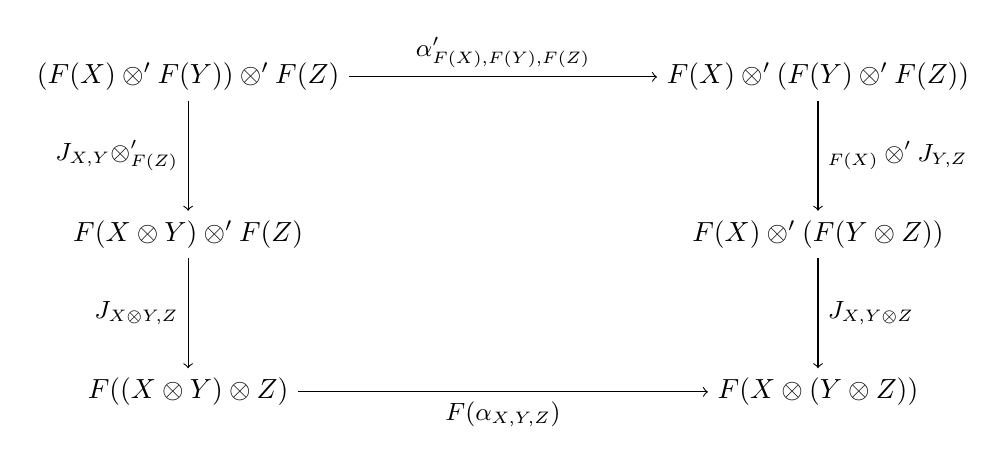
\begin{tikzpicture}
					\node (1) at (0,0) {$(F(X)\otimes'F(Y))\otimes'F(Z)$};
					\node (2) at (8,0) {$F(X)\otimes'(F(Y)\otimes'F(Z))$};
					\node (3) at (0,-2) {$F(X\otimes Y)\otimes'F(Z)$};
					\node (4) at (8,-2) {$F(X)\otimes'(F(Y\otimes Z))$};
					\node (5) at (0,-4) {$F((X\otimes Y)\otimes Z)$};
					\node (6) at (8,-4) {$F(X\otimes (Y\otimes Z))$};
					\draw[->] (1) to node[above] {\small $\alpha'_{F(X),F(Y),F(Z)}$} (2);
					\draw[->] (1) to node[left] {\small $J_{X,Y}\otimes'\id_{F(Z)}$} (3);
					\draw[->] (3) to node[left] {\small $J_{X\otimes Y,Z}$} (5);
					\draw[->] (2) to node[right] {\small $\id_{F(X)}\otimes' J_{Y,Z}$} (4);
					\draw[->] (4) to node[right] {\small $J_{X,Y\otimes Z}$} (6);
					\draw[->] (5) to node[below] {\small $F(\alpha_{X,Y,Z})$} (6);
				\end{tikzpicture}
			\end{figure}
		A monoidal functor is said to be an equivalence of monoidal categories if it is an equivalence of ordinary categories.
	\end{defn}

	\begin{defn}[Strict]
		A monoidal category is strict\index{strict category} if the associativity isomorphism and the unit constraints are identities, hence for all objects $X,Y,Z\in\Obj(\C)$ there are equalities
			\begin{align}
				(X\otimes Y)\otimes Z&=X\otimes(Y\otimes Z)\\
				X\otimes\mathbf{1}&=X=\mathbf{1}\otimes X.
			\end{align}
	\end{defn}

	\begin{thm}
		\label{thm:strictness}
		Every monoidal category is monoidally equivalent to a strict monoidal category.
	\end{thm}

	\begin{proof}
		See \cite[Theorem 2.8.5]{Etingof2015}.
	\end{proof}

	\begin{rem}
		Note that although \cref{thm:strictness} implies you can always turn your category into a strict one, it is not necessarily useful to do so. For example, in order to make a monoidal category strict one may have to add new objects to it (see \cite[Remark 2.8.6]{Etingof2015}). But if you already have an idea of what the objects in your category should be, you might not want to abandon this to make the category strict, even though it would allow you to work with trivial associativity and unit constraints.
	\end{rem}

	\begin{rem}
		Instead of turning your category into a strict one, it is sometimes more useful to turn it into a \emph{skeletal} one. A skeletal\index{skeletal category} category is one which has only one object in every isomorphism class, i.e., if two objects are isomorphic to each other, they are actually equal. Any category is equivalent to a skeletal one (simply by the axiom of choice), however, a monoidal category does not have to be equivalent to a category that is strict and skeletal at the same time. Although the associators are non-trivial in a skeletal category, these categories are still often particularly nice to work with in actual calculations.
	\end{rem}


\subsection*{Graphical calculus of monoidal categories}


Monoidal categories, often equipped with additional structure, come with a graphical language of \emph{string diagrams}. This often helps to visualise and simplify relations and equations in the category. Such a calculus has first been introduced in \cite{Joyal1991} and has been widely used afterwards. Some introductions with different emphases are \cite{kassel_quantum_1995}, \cite{Selinger2010} and \cite{HV19}. The convention we use throughout this thesis is that diagrams are always read from bottom to top (unless otherwise stated).

Given a category $\C$, a morphism $f:X\to Y$ is depicted as a two-dimensional planar diagram
	\begin{equation}
		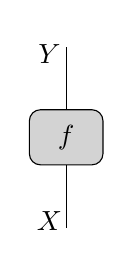
\begin{tikzpicture}[scale=0.85]
			\node (X) at (0,0) {};
			\node (Y) at (0,3) {};
			\node at (-0.25,0.25) {$X$};
			\node at (-0.25,2.75) {$Y$};
			\node [rectangle,draw,text width=0.7cm,minimum height=0.7cm,
			text centered,rounded corners, fill=LightGray, name = f] at (0,1.5) {$f$};
			\draw (X) -- (f);
			\draw (f) -- (Y);
		\end{tikzpicture}
	\end{equation}
\noindent
Every morphism has an ingoing leg (the domain) and an outgoing leg (the codomain). The identity morphism $\id_X:X\to X$ is represented by a straight line:
	\begin{equation}
		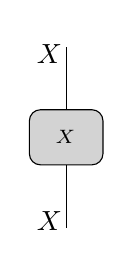
\begin{tikzpicture}[scale=0.85,baseline=(current bounding box.center)]
			\node (X) at (0,0) {};
			\node (Y) at (0,3) {};
			\node at (-0.25,0.25) {$X$};
			\node at (-0.25,2.75) {$X$};
			\node [rectangle,draw,text width=0.7cm,minimum height=0.7cm,
			text centered,rounded corners, fill=LightGray, name = f] at (0,1.5) {$\id_X$};
			\draw (X) -- (f);
			\draw (f) -- (Y);
		\end{tikzpicture}\ \equiv\begin{tikzpicture}[scale=0.85,baseline=(current bounding box.center)]
			\node (X) at (0,0) {};
			\node (Y) at (0,3) {};
			\node at (-0.25,0.25) {$X$};
			\node at (-0.25,2.75) {$X$};
			\draw (X) -- (Y);
		\end{tikzpicture}
	\end{equation}
\noindent
Composition of morphisms corresponds to connecting legs: Given two morphisms $f:X\to Y$ and $g: Y\to Z$, the composed morphism $g\circ f:X\to Z$ is depicted
	\begin{equation}
		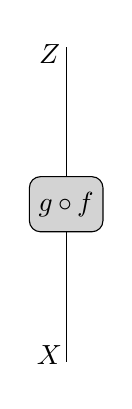
\begin{tikzpicture}[scale=0.85,baseline=(current bounding box.center)]
			\node (X) at (0,0) {};
			\node (Y) at (0,5) {};
			\node at (-0.25,0.25) {$X$};
			\node at (-0.25,4.75) {$Z$};
			\node [rectangle,draw,text width=0.7cm,minimum height=0.7cm,
			text centered,rounded corners, fill=LightGray, name = f] at (0,2.5) {$g\circ f$};
			\draw (X) -- (f);
			\draw (f) -- (Y);
			\end{tikzpicture}\ \ =\ 
		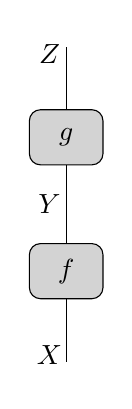
\begin{tikzpicture}[scale=0.85,baseline=(current bounding box.center)]
			\node (X) at (0,0) {};
			\node (Z) at (0,5) {};
			\node at (-0.25,0.25) {$X$};
			\node at (-0.25,2.5) {$Y$};
			\node at (-0.25,4.75) {$Z$};
			\node [rectangle,draw,text width=0.7cm,minimum height=0.7cm,
			text centered,rounded corners, fill=LightGray, name = f] at (0,1.5) {$f$};
			\node [rectangle,draw,text width=0.7cm,minimum height=0.7cm,
			text centered,rounded corners, fill=LightGray, name = g] at (0,3.5) {$g$};
			\draw (X) -- (f);
			\draw (f) -- (g);
			\draw (g) -- (Z);
		\end{tikzpicture}
	\end{equation}
Note that in this graphical calculus associativity of morphisms is implicit. Consider the three morphisms $f:W\to X$, $g:X\to Y$ and $h:Y\to Z$, then both parenthesis structures, $(h\circ g)\circ f$ and $h\circ (g\circ f)$ are depicted
	\begin{figure}[H]
		\centering
		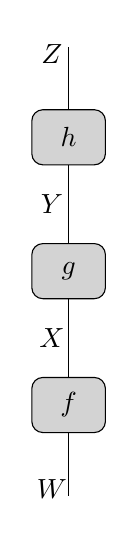
\begin{tikzpicture}[scale=0.85]
			\node (X) at (0,0) {};
			\node (Z) at (0,7) {};
			\node at (-0.25,0.25) {$W$};
			\node at (-0.25,2.5) {$X$};
			\node at (-0.25,4.5) {$Y$};
			\node at (-0.25,6.75) {$Z$};
			\node [rectangle,draw,text width=0.7cm,minimum height=0.7cm,
			text centered,rounded corners, fill=LightGray, name = f] at (0,1.5) {$f$};
			\node [rectangle,draw,text width=0.7cm,minimum height=0.7cm,
			text centered,rounded corners, fill=LightGray, name = g] at (0,3.5) {$g$};
			\node [rectangle,draw,text width=0.7cm,minimum height=0.7cm,
			text centered,rounded corners, fill=LightGray, name = h] at (0,5.5) {$h$};
			\draw (X) -- (f);
			\draw (f) -- (g);
			\draw (g) -- (h);
			\draw (h) -- (Z);
		\end{tikzpicture}
	\end{figure}

The previous diagrams are all valid in any category since they just visualise the concepts and properties mentioned in \cref{def:cat}. More specific to a monoidal category is the visualisation of the monoidal product (or tensor product). Given two morphisms $f:X\to X'$ and $g:Y\to Y'$, their tensor product $f\otimes g:X\otimes Y\to X'\otimes Y'$ is the horizontal juxtaposition of the individual diagrams: 
	\begin{equation}
		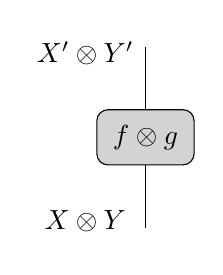
\begin{tikzpicture}[scale=0.85,baseline=(current bounding box.center)]
			\node (X) at (0,0) {};
			\node (Y) at (0,3) {};
			\node at (-0.9,0.25) {$X\otimes Y$};
			\node at (-0.9,2.75) {$X'\otimes Y'$};
			\node [rectangle,draw,text width=1cm,minimum height=0.7cm,
			text centered,rounded corners, fill=LightGray, name = f] at (0,1.5) {$f\otimes g$};
			\draw (X) -- (f);
			\draw (f) -- (Y);
		\end{tikzpicture}\ =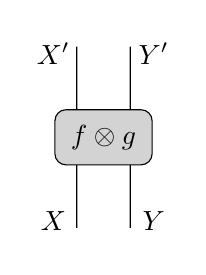
\begin{tikzpicture}[scale=0.85,baseline=(current bounding box.center)]
			\node (X) at (-0.4,0) {};
			\node (Y) at (-0.4,3) {};
			\node (X2) at (0.4,0) {};
			\node (Y2) at (0.4,3) {};
			\node at (-0.75,0.25) {$X$};
			\node at (-0.75,2.75) {$X'$};
			\node at (0.75,0.25) {$Y$};
			\node at (0.75,2.75) {$Y'$};
			\draw (X) -- (-0.4,1.5);
			\draw (-0.4,1.5) -- (Y);
			\draw (X2) -- (0.4,1.5);
			\draw (0.4,1.5) -- (Y2);
			\node [rectangle,draw,text width=1cm,minimum height=0.7cm,
			text centered,rounded corners, fill=LightGray, name = f] at (0,1.5) {$f\otimes g$};
		\end{tikzpicture}\ =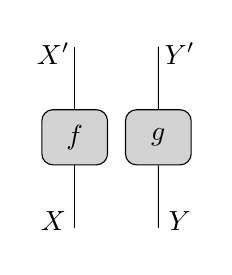
\begin{tikzpicture}[scale=0.85,baseline=(current bounding box.center)]
			\node (X) at (0,0) {};
			\node (Y) at (0,3) {};
			\node at (-0.25,0.25) {$X\ $};
			\node at (-0.25,2.75) {$X'\ $};
			\node [rectangle,draw,text width=0.6cm,minimum height=0.7cm,
			text centered,rounded corners, fill=LightGray, name = f] at (0,1.5) {$f$};
			\draw (X) -- (f);
			\draw (f) -- (Y);
			\node (X) at (1.25,0) {};
			\node (Y) at (1.25,3) {};
			\node at (1.5,0.25) {$\ Y$};
			\node at (1.5,2.75) {$\ Y'$};
			\node [rectangle,draw,text width=0.6cm,minimum height=0.7cm,
			text centered,rounded corners, fill=LightGray, name = f] at (1.25,1.5) {$g$};
			\draw (X) -- (f);
			\draw (f) -- (Y);
		\end{tikzpicture}
	\end{equation}
The unit object $\mathbf{1}$ is often depicted either as a dashed line or by the absence of any line when it is clear from the context, e.g., the morphism $f:\mathbf{1}\to X\otimes Y$ can be drawn in the following ways:
	\begin{equation}
		\begin{tikzpicture}[scale=0.85,baseline=(current bounding box.center)]
			\node (X) at (-0.4,0) {};
			\node (Y) at (-0.4,3) {};
			\node (X2) at (0,0) {};
			\node at (-0.75,2.75) {$X$};
			\node at (0.75,2.75) {$Y$};
			\node at (-0.25,0.25) {$\mathbf{1}$};
			\draw (-0.4,1.5) -- (Y);
			\draw (0.4,1.5) -- (Y2);
			\node [rectangle,draw,text width=0.9cm,minimum height=0.7cm,
			text centered,rounded corners, fill=LightGray, name = f] at (0,1.5) {$f$};
			\draw (X2) -- (f);
		\end{tikzpicture}\ =\begin{tikzpicture}[scale=0.85,baseline=(current bounding box.center)]
			\node (X) at (-0.4,0) {};
			\node (Y) at (-0.4,3) {};
			\node (X2) at (0,0) {};
			\node at (-0.75,2.75) {$X$};
			\node at (0.75,2.75) {$Y$};
%			\node at (-0.25,0.25) {$\mathbf{1}$};
			\draw (-0.4,1.5) -- (Y);
			\draw (0.4,1.5) -- (Y2);
			\node [rectangle,draw,text width=0.9cm,minimum height=0.7cm,
			text centered,rounded corners, fill=LightGray, name = f] at (0,1.5) {$f$};
			\draw[dashed] (X2) -- (f);
		\end{tikzpicture}\ =\begin{tikzpicture}[scale=0.85,baseline=(current bounding box.center)]
			\node (X) at (-0.4,0) {};
			\node (Y) at (-0.4,3) {};
			\node (X2) at (0,0) {};
			\node at (-0.75,2.75) {$X$};
			\node at (0.75,2.75) {$Y$};
			\node at (-0.25,0.25) {};
			\draw (-0.4,1.5) -- (Y);
			\draw (0.4,1.5) -- (Y2);
			\node [rectangle,draw,text width=0.9cm,minimum height=0.7cm,
			text centered,rounded corners, fill=LightGray, name = f] at (0,1.5) {$f$};
		\end{tikzpicture}
	\end{equation}

We will use and extend the here presented graphical calculus in the following sections to illustrate different concepts and properties of categories, such as duals of morphisms and braiding structures, and to explain calculations within them, e.g., how to define and evaluate the trace of an object or a morphism graphically.


\section{Fusion categories}
\label{sec:fusioncat}

Fusion categories are monoidal categories that are especially easy to work with since the morphism spaces are linear vector spaces and all properties can be expressed in terms of the simple objects of the category. However, before we state the definition of a fusion category, we need to introduce several adjectives.

	\begin{defn}[Left duals]
		In a monoidal category $(\C,\otimes,\alpha,\mathbf{1},l,r)$, an object $X^*\in\Obj(\C)$ is said to be a left dual\index{left dual} of $X\in\Obj(\C)$ if there exist morphisms
			\begin{align}
				\ev_X&:X^*\otimes X\to\mathbf{1}\\
				\coev_X&:\mathbf{1}\to X\otimes X^*,
			\end{align}
		depicted
			\begin{align}
				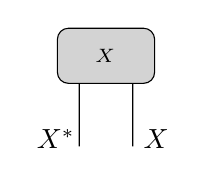
\begin{tikzpicture}[scale=0.85,baseline=(current bounding box.center)]
					\node (X) at (-0.4,0) {};
					\node (X2) at (0.4,0) {};
					\node at (-0.75,0.25) {$X^*$};
					\node at (0.75,0.25) {$X$};
					\draw (X) -- (-0.4,1.5);
					\draw (X2) -- (0.4,1.5);
					\node [rectangle,draw,text width=1cm,minimum height=0.7cm,
					text centered,rounded corners, fill=LightGray, name = f] at (0,1.5) {$\ev_X$};
				\end{tikzpicture}\ =
				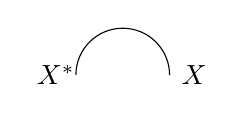
\begin{tikzpicture}[scale=0.85,baseline=(current bounding box.center)]
					\node at (-0.3,0) {$X^*$};
					\node at (1.7,0) {$\ X$};
					\draw (0,0) arc (180:0:0.7);
				\end{tikzpicture}\hspace{20pt}
				\begin{tikzpicture}[scale=0.85,baseline=(current bounding box.center)]
					\node (X) at (-0.4,0) {};
					\node (Y) at (-0.4,3) {};
					\node (X2) at (0,0) {};
					\node at (-0.75,2.75) {$X$};
					\node at (0.75,2.75) {$X^*$};
					\node at (-0.25,0.25) {};
					\draw (-0.4,1.5) -- (Y);
					\draw (0.4,1.5) -- (Y2);
					\node [rectangle,draw,text width=0.9cm,minimum height=0.7cm,
					text centered,rounded corners, fill=LightGray, name = f] at (0,1.5) {$\coev_X$};
				\end{tikzpicture}=
				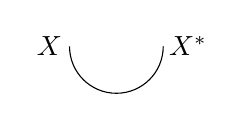
\begin{tikzpicture}[scale=0.85,baseline=(current bounding box.center)]
					\node at (-0.3,0) {$X$};
					\node at (1.7,0) {$\ X^*$};
					\draw (0,0) arc (-180:0:0.7);
				\end{tikzpicture}
			\end{align}
		such that the compositions
			\begin{align}
				X\xrightarrow{\coev_X\otimes\,\id_X}(X\otimes X^*)\otimes X&\xrightarrow{a_{X,X^*,X}}X\otimes(X^*\otimes X)\xrightarrow{\id_X\otimes\,\ev_X}X\\
				X^*\xrightarrow{\id_{X^*}\otimes\,\coev_X}X^*\otimes(X\otimes X^*)&\xrightarrow{a_{X^*,X,X^*}^{-1}}(X^*\otimes X)\otimes X^*\xrightarrow{\ev_X\otimes\,\id_{X^*}}X^*
			\end{align}
		are the identity morphisms, which is equivalent to the following equations: 
			\begin{align}
				\begin{tikzpicture}[baseline=(current bounding box.center)]
					\draw (0,0) -- (0,1);
					\draw (0,1) arc (0:180:0.4);
					\draw (-0.8,1) arc (0:-180:0.4);
					\draw (-1.6,1) -- (-1.6,2);
					\node at (0.25,0) {$X$};
					\node at (-1.85,2) {$X$};
					\node at (-1.05,1) {$X^*$};
				\end{tikzpicture}\ =
				\begin{tikzpicture}[baseline=(current bounding box.center)]
					\draw (0,0) -- (0,2);
					\node at (-0.25,0)  {$X$};
					\node at (-0.25,2) {\phantom{$X$}};
				\end{tikzpicture}\hspace{50pt}
				\begin{tikzpicture}[baseline=(current bounding box.center)]
					\draw (0,0) -- (0,1);
					\draw (0,1) arc (180:0:0.4);
					\draw (0.8,1) arc (-180:0:0.4);
					\draw (1.6,1) -- (1.6,2);
					\node at (-0.25,0) {$X^*$};
					\node at (1.85,2) {$\ X^*$};
					\node at (1.05,1) {$X$};
				\end{tikzpicture}\ =
				\begin{tikzpicture}[baseline=(current bounding box.center)]
					\draw (0,0) -- (0,2);
					\node at (-0.25,0)  {$X^*$};
					\node at (-0.25,2) {\phantom{$X^*$}};
				\end{tikzpicture}\ .
			\end{align}
		These morphisms are called evaluation\index{evaluation} and coevaluation\index{coevaluation}.
	\end{defn}

	\begin{defn}[Right duals]
		In a monoidal category $(\C,\otimes,\alpha,\mathbf{1},l,r)$, an object $\lstar X\in\Obj(\C)$ is said to be a right dual\index{right dual} of $X\in\Obj(\C)$ if there exist morphisms
		\begin{align}
		\ev_X'&:X\otimes \lstar X\to\mathbf{1}\\
		\coev_X'&:\mathbf{1}\to \lstar X\otimes X,
		\end{align}
		depicted
			\begin{align}
				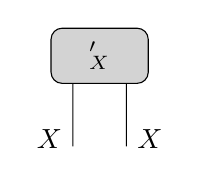
\begin{tikzpicture}[scale=0.85,baseline=(current bounding box.center)]
				\node (X) at (-0.4,0) {};
				\node (X2) at (0.4,0) {};
				\node at (-0.75,0.25) {$X$};
				\node at (0.75,0.25) {$\lstar X$};
				\draw (X) -- (-0.4,1.5);
				\draw (X2) -- (0.4,1.5);
				\node [rectangle,draw,text width=1cm,minimum height=0.7cm,
				text centered,rounded corners, fill=LightGray, name = f] at (0,1.5) {$\ev'_X$};
				\end{tikzpicture}\ =
				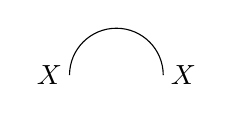
\begin{tikzpicture}[scale=0.85,baseline=(current bounding box.center)]
				\node at (-0.3,0) {$X$};
				\node at (1.7,0) {$\lstar X$};
				\draw (0,0) arc (180:0:0.7);
				\end{tikzpicture}\hspace{20pt}
				\begin{tikzpicture}[scale=0.85,baseline=(current bounding box.center)]
				\node (X) at (-0.4,0) {};
				\node (Y) at (-0.4,3) {};
				\node (X2) at (0,0) {};
				\node at (-0.75,2.75) {$\lstar X$};
				\node at (0.75,2.75) {$X$};
				\node at (-0.25,0.25) {};
				\draw (-0.4,1.5) -- (Y);
				\draw (0.4,1.5) -- (Y2);
				\node [rectangle,draw,text width=0.9cm,minimum height=0.7cm,
				text centered,rounded corners, fill=LightGray, name = f] at (0,1.5) {$\coev'_X$};
				\end{tikzpicture}=
				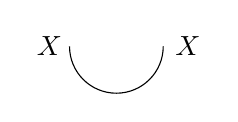
\begin{tikzpicture}[scale=0.85,baseline=(current bounding box.center)]
				\node at (-0.3,0) {$\lstar X$};
				\node at (1.7,0) {$\ X$};
				\draw (0,0) arc (-180:0:0.7);
				\end{tikzpicture}
			\end{align}
		such that the compositions
		\begin{align}
		X\xrightarrow{\id_X\otimes\,\coev_X'}X\otimes(\lstar X\otimes X)&\xrightarrow{a_{X,\lstar X,X}^{-1}}(X\otimes{}^*X)\otimes X\xrightarrow{\ev_X'\otimes\,\id_X}X\\
	\lstar X\xrightarrow{\coev_X'\otimes\,\id_{\lstar X}}(\lstar X\otimes X)\otimes \lstar X&\xrightarrow{a_{\lstar X,X,\lstar X}}\lstar X\otimes (X\otimes \lstar X)\xrightarrow{\id_{\lstar X}\otimes\,\ev_{X}'}\lstar X
		\end{align}
		are the identity morphisms, which is equivalent to the following equations:
			\begin{align}
				\begin{tikzpicture}[baseline=(current bounding box.center)]
					\draw (0,0) -- (0,1);
					\draw (0,1) arc (180:0:0.4);
					\draw (0.8,1) arc (-180:0:0.4);
					\draw (1.6,1) -- (1.6,2);
					\node at (-0.25,0) {$X$};
					\node at (1.85,2) {$\ X$};
					\node at (1.05,1) {$\ \lstar X$};
				\end{tikzpicture}\ =
				\begin{tikzpicture}[baseline=(current bounding box.center)]
					\draw (0,0) -- (0,2);
					\node at (-0.25,0)  {$X$};
					\node at (-0.25,2) {\phantom{$X$}};
				\end{tikzpicture}\hspace{50pt}
				\begin{tikzpicture}[baseline=(current bounding box.center)]
					\draw (0,0) -- (0,1);
					\draw (0,1) arc (0:180:0.4);
					\draw (-0.8,1) arc (0:-180:0.4);
					\draw (-1.6,1) -- (-1.6,2);
					\node at (0.25,0) {$\ \lstar X$};
					\node at (-1.85,2) {$\lstar X$};
					\node at (-1.05,1) {$X$};
				\end{tikzpicture}\ =
				\begin{tikzpicture}[baseline=(current bounding box.center)]
					\draw (0,0) -- (0,2);
					\node at (-0.25,0)  {$\lstar X$};
					\node at (-0.25,2) {\phantom{$\lstar X$}};
				\end{tikzpicture}
			\end{align}
	\end{defn}

	\begin{rem}
		Note that for an object $X\in\Obj(\C)$, the left (respectively, right) dual object is unique up to a unique isomorphism.
	\end{rem}

	\begin{rem}
		If $X^*\in\C$ is a left dual of an object $X\in\C$, then it is obvious that $X$ is a right dual of $X^*$ with $\ev'_{X^*}=\ev_X$ and $\coev'_{X^*}=\coev_X$, and vice versa. This implies that $\lstar (X^*)\cong X\cong (\lstar X)^*$ for any object in $\C$ with left and right duals. Furthermore, in any monoidal category, it holds that $\mathbf{1}^*=\lstar \mathbf{1}=\mathbf{1}$.
	\end{rem}

	\begin{rem}
		\label{rem:dualmorphs}
		We can use the definitions of evaluation and coevaluation to construct duals of morphisms: If $X$ and $Y$ are objects in a category $\C$ that have left duals $X^*,Y^*$, and $f:X\to Y$ is a morphism between them, one defines the left dual $f^*:Y^*\to X^*$ of $f$ by the composition
			\begin{align}
				f^*\equiv Y^*\xrightarrow{\id_{Y^*}\otimes\coev_X}Y^*\otimes (X\otimes X^*)\xrightarrow{\alpha_{Y^*,X,X^*}^{-1}}(Y^*\otimes X)\otimes &X^*\\
				\xrightarrow{(\id_Y\otimes f)\otimes \id_{X^*}}(Y^*\otimes Y)\otimes X^*\xrightarrow{\ev_Y\otimes\id_{X^*}}&X^*.
			\end{align}
		Using graphical notation, the dual morphism\index{dual morphism} $f^*$ is depicted
			\begin{equation}
			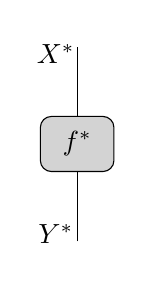
\begin{tikzpicture}[scale=0.85,baseline=(current bounding box.center)]
				\node (X) at (0,0.9) {};
				\node (Y) at (0,4.1) {};
				\node at (-0.25,1.15) {$Y^*\ $};
				\node at (-0.25,3.85) {$X^*\ $};
				\node [rectangle,draw,text width=0.7cm,minimum height=0.7cm,
				text centered,rounded corners, fill=LightGray, name = f] at (0,2.5) {$f^*$};
				\draw (X) -- (f);
				\draw (f) -- (Y);
			\end{tikzpicture}\ \ =\ 
			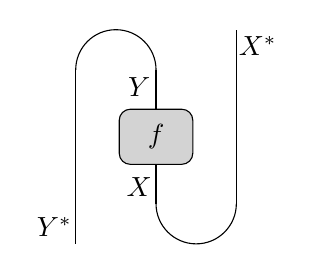
\begin{tikzpicture}[scale=0.85,baseline=(current bounding box.center)]
				\node at (-0.25,1.75) {$X$};
				\node at (-0.25,3.25) {$Y$};
				\node [rectangle,draw,text width=0.7cm,minimum height=0.7cm,
				text centered,rounded corners, fill=LightGray, name = f] at (0,2.5) {$f$};
				\draw (0,1.5) -- (f);
				\draw (f) -- (0,3.5);
				\draw (0,1.5) arc (-180:0:0.6);
				\draw (0,3.5) arc (0:180:0.6);
				\draw (1.2,1.5) -- (1.2,4.1);
				\draw (-1.2,3.5) -- (-1.2,0.9);
				\node at (-1.45,1.15) {$Y^*\ $};
				\node at (1.45,3.85) {$\ X^*$};
			\end{tikzpicture}
			\end{equation}
		Analogously, if $X,Y\in\Obj(\C)$ have right duals $\lstar X,\lstar Y$ and $f:X\to Y$ is a morphism, one defines the right dual $\lstar f:\lstar Y\to\lstar X$ of $f$ by
			\begin{align}
				\lstar f\equiv\lstar Y\xrightarrow{\coev'_X\otimes\id_{\lstar Y}}(\lstar X\otimes X)\otimes \lstar Y\xrightarrow{\alpha_{\lstar X,X,\lstar Y}}\lstar X\otimes (X\otimes \lstar Y&)\\\xrightarrow{\id_{\lstar X}\otimes(f\otimes\id_{\lstar Y})}\lstar X\otimes(Y\otimes \lstar Y)\xrightarrow{\id_{\lstar X}\otimes\ev'_{Y}}\lstar X&,
			\end{align}
		which is graphically
			\begin{equation}
			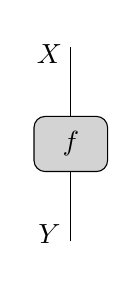
\begin{tikzpicture}[scale=0.85,baseline=(current bounding box.center)]
				\node (X) at (0,0.9) {};
				\node (Y) at (0,4.1) {};
				\node at (-0.25,1.15) {$\lstar Y\ $};
				\node at (-0.25,3.85) {$\lstar X\ $};
				\node [rectangle,draw,text width=0.7cm,minimum height=0.7cm,
				text centered,rounded corners, fill=LightGray, name = f] at (0,2.5) {$\lstar f$};
				\draw (X) -- (f);
				\draw (f) -- (Y);
			\end{tikzpicture}\ \ =\ 
			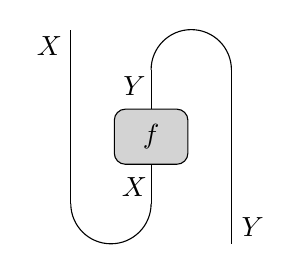
\begin{tikzpicture}[scale=0.85,baseline=(current bounding box.center)]
				\node at (-0.25,1.75) {$X$};
				\node at (-0.25,3.25) {$Y$};
				\node [rectangle,draw,text width=0.7cm,minimum height=0.7cm,
				text centered,rounded corners, fill=LightGray, name = f] at (0,2.5) {$f$};
				\draw (0,1.5) -- (f);
				\draw (f) -- (0,3.5);
				\draw (0,1.5) arc (0:-180:0.6);
				\draw (0,3.5) arc (180:0:0.6);
				\draw (-1.2,1.5) -- (-1.2,4.1);
				\draw (1.2,3.5) -- (1.2,0.9);
				\node at (-1.45,3.85) {$\lstar X\ $};
				\node at (1.45,1.15) {$\ \lstar Y$};
			\end{tikzpicture}
			\end{equation}
	\end{rem}

	\begin{defn}[Rigid]
		An object in a monoidal category is called rigid\index{rigid category} if it has left and right duals. A monoidal category $\C$ is called rigid if every object of $\C$ is rigid.
	\end{defn}
	
	\begin{defn}[$k$-linear]
		Let $k$ be a field. A category $\C$ is said to be $k$-linear\index{k-linear category@$k$-linear category} if for all objects $X,Y\in\Obj(\C)$ the morphisms $\Hom(X,Y)$ form a $k$-vector space and the composition of morphisms in $\C$ is bilinear with respect to $k$.
	\end{defn}
	
	\begin{defn}[Simple and semisimple]
		Let $\C$ be a $k$-linear category. An object $X\in\Obj(\C)$ is called simple\index{simple object} if $\Hom(X,X)=k$. An object is called semisimple\index{semisimple object} if it can be written as a direct sum\footnote{A monoidal category $\C$ is always equipped with a bifunctor $\oplus:\C\times\C\to\C$ that ensures that the direct sum $X_1\oplus X_2$ of two objects in the category is again an object in the category.} of simple objects. A category $\C$ is called semisimple\index{semisimple category} if every object of $\C$ is semisimple.
	\end{defn}
	
	\begin{defn}[Fusion category]
		\label{def:fusioncat}
		A fusion category\index{fusion category} over $\mathbb{C}$ is a $\mathbb{C}$-linear rigid semisimple monoidal category with finitely many simple objects (up to isomorphism) and finite-dimensional morphism spaces such that the identity object is simple.
	\end{defn}

	\begin{rem}
		\label{rem:multiplicities}
		Semisimplicity makes it easy to talk about properties of the category since, generally speaking, everything can be characterized by its action on the simple objects. Furthermore, for a fusion category $\C$, semisimplicity allows us to define multiplicity coefficients in the following way: Label the equivalence classes of simple objects by some set $I$ and choose a representative $X_i$ for each equivalence class $i\in I$. For $i,j\in I$ there are then integers $N_{ij}^k\in\mathbb{Z}_+$ such that
			\begin{equation}
				\label{eq:fusionrule}
				X_i\otimes X_j=\bigoplus_{k\in I} N_{ij}^k X_k.
			\end{equation}
		The notation $N X_k$ denotes the direct sum of $N$ copies of the object $X_k$. We will use these coefficients later in physical applications, where \cref{eq:fusionrule} is called a \emph{fusion rule}\footnote{The name \emph{fusion rule} originates from conformal field theory, where it describes how two excitations can fuse (see \cite{Verlinde1988}).}\index{fusion rule} and the multiplicities $N_{ij}^k$\index{multiplicities} are referred to as \emph{fusion coefficients}\index{fusion coefficients} (see \cref{sec:anyons}). A fusion category is said to be \emph{multiplicity-free}\index{multiplicity-free} if $N_{ij}^k\in\{0,1\}$ for all choices of $i,j,k$.
	\end{rem}

\subsection*{Working in a basis: $F$-symbols for fusion categories}

When studying physical systems in Part $2$ of this thesis, we often choose a basis to do calculations in. This is especially convenient since this means that most of our calculations can be done in terms of matrices and vectors, hence we only need to employ linear algebra. When working in a basis, an important part of the data of a fusion category are $F$-symbols (also called $6j$-symbols). Here, also the notion of fusion coefficients introduced in \cref{rem:multiplicities} comes in handy.

For reasons of clarity, we use a more convenient notation for the morphism space of a trivalent vertex 
	\begin{tikzpicture}[scale=0.9,baseline=(current bounding box.center)]
		\draw (0,0) -- (150:0.3);
		\draw (0,0) -- (270:0.3);
		\draw (0,0) -- (30:0.3);
		\node at (150:0.45) {\scriptsize $a$};
		\node at (270:0.45) {\scriptsize $u$};
		\node at (30:0.45) {\scriptsize $b$};
	\end{tikzpicture} 
in the following:
	\begin{equation}
		V_u^{ab}\equiv\Hom(u,a\otimes b),
	\end{equation}
When considering a tensor product of three objects instead of two, there are two ways of decomposing the morphism space $V_u^{abc}$: 
	\begin{align}
		V_u^{abc}&=\bigoplus_p V_p^{ab}\otimes V_u^{pc},\\
		V_u^{abc}&=\bigoplus_q V_u^{aq}\otimes V_q^{bc},
	\end{align}
where the first decomposition corresponds to morphisms given by diagrams of the form
	\begin{equation}
		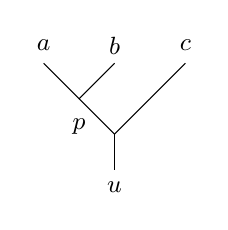
\begin{tikzpicture}[baseline=(current bounding box.center),scale=0.9]
			\draw (0,0.5) -- (0,1);
			\draw (0,1) -- (-0.5,1.5);
			\draw (-0.5,1.5) -- (-1,2);
			\draw (-0.5,1.5) -- (0,2);
			\draw (0,1) -- (0.5,1.5);
			\draw (0.5,1.5) -- (1,2);
			\node at (0,0.25) {\small $u$};
			\node at (-1,2.25) {\small $a$};
			\node at (0,2.25) {\small $b$};
			\node at (1,2.25) {\small $c$};
			\node at (-0.5,1.1) {\small $p$};
		\end{tikzpicture},
	\end{equation}
and the second decomposition of the space corresponds to diagrams of the form
	\begin{equation}
		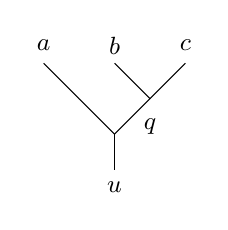
\begin{tikzpicture}[baseline=(current bounding box.center),yscale=0.9,xscale=0.9]
			\draw (0,0.5) -- (0,1);
			\draw (0,1) -- (-0.5,1.5);
			\draw (-0.5,1.5) -- (-1,2);
			\draw (0.5,1.5) -- (0,2);
			\draw (0,1) -- (0.5,1.5);
			\draw (0.5,1.5) -- (1,2);
			\node at (0,0.25) {\small $u$};
			\node at (-1,2.25) {\small $a$};
			\node at (0,2.25) {\small $b$};
			\node at (1,2.25) {\small $c$};
			\node at (0.5,1.1) {\small $q$};
		\end{tikzpicture}.
	\end{equation}
These two choices are connected via a unitary isomorphism which is given by the so-called $F$-symbol\footnote{We also use the terms $F$-move and $F$-matrix in the following.}\index{F-symbol@$F$-symbol}. This is a map between the two different decompositions of $V_u^{abc}$:
	\begin{equation}
		F_u^{abc}:\bigoplus_p V_p^{ab}\otimes V_u^{pc}\to \bigoplus_q V_u^{aq}\otimes V_q^{bc},
	\end{equation}
whose matrix elements are given as follows:
	\begin{equation}
		\label{eq:Fmove}
		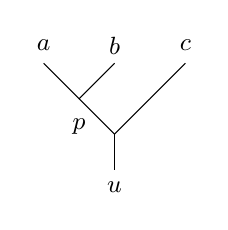
\begin{tikzpicture}[baseline=(current bounding box.center),yscale=0.9,xscale=0.9]
			\draw (0,0.5) -- (0,1);
			\draw (0,1) -- (-0.5,1.5);
			\draw (-0.5,1.5) -- (-1,2);
			\draw (-0.5,1.5) -- (0,2);
			\draw (0,1) -- (0.5,1.5);
			\draw (0.5,1.5) -- (1,2);
			\node at (0,0.25) {\small $u$};
			\node at (-1,2.25) {\small $a$};
			\node at (0,2.25) {\small $b$};
			\node at (1,2.25) {\small $c$};
			\node at (-0.5,1.1) {\small $p$};
		\end{tikzpicture}=\sum_q \left(F_u^{abc}\right)_{qp}
		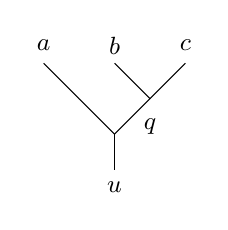
\begin{tikzpicture}[baseline=(current bounding box.center),yscale=0.9,xscale=0.9]
			\draw (0,0.5) -- (0,1);
			\draw (0,1) -- (-0.5,1.5);
			\draw (-0.5,1.5) -- (-1,2);
			\draw (0.5,1.5) -- (0,2);
			\draw (0,1) -- (0.5,1.5);
			\draw (0.5,1.5) -- (1,2);
			\node at (0,0.25) {\small $u$};
			\node at (-1,2.25) {\small $a$};
			\node at (0,2.25) {\small $b$};
			\node at (1,2.25) {\small $c$};
			\node at (0.5,1.1) {\small $q$};
		\end{tikzpicture}.
	\end{equation}
The $F$-matrix $F_u^{abc}$ corresponds to a basis-change matrix of $\Hom(u,a\otimes b\otimes c)$ if the category is strict (i.e., the associator $\alpha_{XYZ}:(X\otimes Y)\otimes Z\to X\otimes(Y\otimes Z)$ is the identity), or to an identification $\Hom(u,(a\otimes b)\otimes c)\cong\Hom(u,a\otimes(b\otimes c))$ if the category is not strict.

If the fusion rules of the underlying category are \emph{not} multiplicity-free, we have to consider a few more indices here. The formula in \cref{eq:Fmove} then reads
	\begin{equation}
	\label{eq:Fmovemult}
		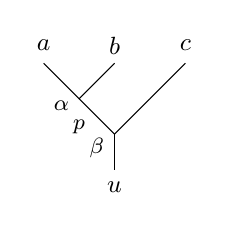
\begin{tikzpicture}[baseline=(current bounding box.center),yscale=0.9,xscale=0.9]
			\draw (0,0.5) -- (0,1);
			\draw (0,1) -- (-0.5,1.5);
			\draw (-0.5,1.5) -- (-1,2);
			\draw (-0.5,1.5) -- (0,2);
			\draw (0,1) -- (0.5,1.5);
			\draw (0.5,1.5) -- (1,2);
			\node at (0,0.25) {\small $u$};
			\node at (-1,2.25) {\small $a$};
			\node at (0,2.25) {\small $b$};
			\node at (1,2.25) {\small $c$};
			\node at (-0.5,1.1) {\footnotesize $p$};
			\node at (-0.75,1.4) {\footnotesize $\alpha$};
			\node at (-0.25,0.8) {\footnotesize $\beta$};
		\end{tikzpicture}=\sum_{q,\gamma,\delta} \left(F_u^{abc}\right)_{(q,\gamma,\delta)(p,\alpha,\beta)}
		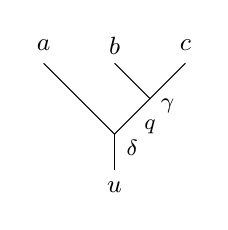
\begin{tikzpicture}[baseline=(current bounding box.center),yscale=0.9,xscale=0.9]
			\draw (0,0.5) -- (0,1);
			\draw (0,1) -- (-0.5,1.5);
			\draw (-0.5,1.5) -- (-1,2);
			\draw (0.5,1.5) -- (0,2);
			\draw (0,1) -- (0.5,1.5);
			\draw (0.5,1.5) -- (1,2);
			\node at (0,0.25) {\small $u$};
			\node at (-1,2.25) {\small $a$};
			\node at (0,2.25) {\small $b$};
			\node at (1,2.25) {\small $c$};
			\node at (0.5,1.1) {\footnotesize $q$};
			\node at (0.75,1.4) {\footnotesize $\gamma$};
			\node at (0.25,0.8) {\footnotesize $\delta$};
		\end{tikzpicture}.
	\end{equation}
In the following, we restrict our studies to the multiplicity-free case.

\begin{figure}[t]
	\centering
	\begin{tikzpicture}[scale=0.7]
	\draw (0,0.25) -- (0,1);
	\draw (0,1) -- (-0.5,1.5);
	\draw (0,1) -- (0.5,1.5);
	\draw (0.5,1.5) -- (1,2);
	\draw (1,2) -- (1.5,2.5);
	\draw (-0.5,1.5) -- (-1,2);
	\draw (-1,2) -- (-1.5,2.5);
	\draw (-0.5,1.5) -- (0,2);
	\draw (0,2) -- (0.5,2.5);
	\draw (-1,2) -- (-0.5,2.5);
	\node at (0,-0.15) {\small $u$};
	\node at (-1.5,2.75) {\small $a$};
	\node at (-0.5,2.75) {\small $b$};
	\node at (0.5,2.75) {\small $c$};
	\node at (1.5,2.75) {\small $d$};
	\node at (-0.9,1.5) {\small $p$};
	\node at (-0.4,1) {\small $q$};
	\draw[->,>=stealth] (2,2) to node[above] {\small $F_{u}^{pcd}$\ } (4.5,3);
	\draw[->,>=stealth] (7.5,3) to node[above] {\small\ \ $F_{u}^{abr}$} (10,2);
	\draw[->,>=stealth] (0.75,0) to node[right,pos=0.3] {\small \ \ $F_{q}^{abc}$} (2,-1.25);
	\draw[->,>=stealth] (10,-1.25) to node[left,pos=0.7] {\small $F_{s}^{bcd}$\ \ } (11.25,0);
	\draw[->,>=stealth] (4.75,-3.5) to node[above] {\small $F_{u}^{atd}$} (7.25,-3.5);
	\begin{scope}[xshift=6cm,yshift=2.5cm]
	\draw (0,0.25) -- (0,1);
	\draw (0,1) -- (-0.5,1.5);
	\draw (0,1) -- (0.5,1.5);
	\draw (0.5,1.5) -- (1,2);
	\draw (1,2) -- (1.5,2.5);
	\draw (-0.5,1.5) -- (-1,2);
	\draw (-1,2) -- (-1.5,2.5);
	\draw (1,2) -- (0.5,2.5);
	\draw (-1,2) -- (-0.5,2.5);
	\node at (0,-0.15) {\small $u$};
	\node at (-1.5,2.75) {\small $a$};
	\node at (-0.5,2.75) {\small $b$};
	\node at (0.5,2.75) {\small $c$};
	\node at (1.5,2.75) {\small $d$};
	\node at (-0.9,1.5) {\small $p$};
	\node at (0.9,1.5) {\small $r$};
	\end{scope}
	\begin{scope}[xshift=12cm]
	\draw (0,0.25) -- (0,1);
	\draw (0,1) -- (-0.5,1.5);
	\draw (0,1) -- (0.5,1.5);
	\draw (0.5,1.5) -- (1,2);
	\draw (1,2) -- (1.5,2.5);
	\draw (-0.5,1.5) -- (-1,2);
	\draw (-1,2) -- (-1.5,2.5);
	\draw (1,2) -- (0.5,2.5);
	\draw (0.5,1.5) -- (0,2);
	\draw (0,2) -- (-0.5,2.5);
	\node at (0,-0.15) {\small $u$};
	\node at (-1.5,2.75) {\small $a$};
	\node at (-0.5,2.75) {\small $b$};
	\node at (0.5,2.75) {\small $c$};
	\node at (1.5,2.75) {\small $d$};
	\node at (0.4,1) {\small $s$};
	\node at (0.9,1.5) {\small $r$};
	\end{scope}
	\begin{scope}[xshift=3.25cm,yshift=-4.5cm]
	\draw (0,0.25) -- (0,1);
	\draw (0,1) -- (-0.5,1.5);
	\draw (0,1) -- (0.5,1.5);
	\draw (0.5,1.5) -- (1,2);
	\draw (1,2) -- (1.5,2.5);
	\draw (-0.5,1.5) -- (-1,2);
	\draw (-1,2) -- (-1.5,2.5);
	\draw (-0.5,1.5) -- (0,2);
	\draw (0,2) -- (0.5,2.5);
	\draw (0,2) -- (-0.5,2.5);
	\node at (0,-0.15) {\small $u$};
	\node at (-1.5,2.75) {\small $a$};
	\node at (-0.5,2.75) {\small $b$};
	\node at (0.5,2.75) {\small $c$};
	\node at (1.5,2.75) {\small $d$};
	\node at (0.15,1.65) {\small $t$};
	\node at (-0.4,1) {\small $q$};
	\end{scope}
	\begin{scope}[xshift=8.75cm,yshift=-4.5cm]
	\draw (0,0.25) -- (0,1);
	\draw (0,1) -- (-0.5,1.5);
	\draw (0,1) -- (0.5,1.5);
	\draw (0.5,1.5) -- (1,2);
	\draw (1,2) -- (1.5,2.5);
	\draw (-0.5,1.5) -- (-1,2);
	\draw (-1,2) -- (-1.5,2.5);
	\draw (0.5,1.5) -- (0,2);
	\draw (0,2) -- (0.5,2.5);
	\draw (0,2) -- (-0.5,2.5);
	\node at (0,-0.15) {\small $u$};
	\node at (-1.5,2.75) {\small $a$};
	\node at (-0.5,2.75) {\small $b$};
	\node at (0.5,2.75) {\small $c$};
	\node at (1.5,2.75) {\small $d$};
	\node at (0,1.65) {\small $t$};
	\node at (0.45,1) {\small $s$};
	\end{scope}
	\end{tikzpicture}
	\caption{\small \label{fig:PentagonId}\textbf{Pentagon identity in terms of tree diagrams.} To ensure the consistency of the underlying anyon model, this diagram has to commute.}
\end{figure}

We can continue this train of thought by considering morphism spaces with four objects $\Hom(u,a\otimes b\otimes c\otimes d)$. In this case, there are five different possible decompositions of the morphism space $V_u^{abcd}$. With the same argument as above they have to be connected by a unitary isomorphism. As one can see in \cref{fig:PentagonId}, these isomorphisms are again given by the $F$-moves defined in \cref{eq:Fmove}. However, since now we have more possible decompositions than in the previous case, there are several ways to map from one decomposition to another. For instance, consider the leftmost diagram in \cref{fig:PentagonId}. By employing two $F$-moves (upper path), we can completely reverse the order of splitting and transform the diagram into the rightmost one. However, this is also possible by following the lower path in the diagram that includes three $F$-moves. Therefore, to guarantee the consistency of the fusion category, the two paths have to be identical, or, stated differently, the diagram in \cref{fig:PentagonId} has to commute.

Note that every $F$-move in \cref{fig:PentagonId} only acts on a subtree that is determined by its indices. For instance, the $F$-move that maps from the leftmost tree to the upper middle one acts on the subtree that represents the morphism space $\Hom(u,p\otimes c\otimes d)$, while the subtree representing $\Hom(p,a\otimes b)$ remains unchanged. Hence, there is an additional identity acting on $V_p^{ab}$ that we have omitted here for clarity. This becomes clearer when considering the vector space decompositions where the $F$-moves are applied to as depicted in \cref{fig:pentavec}. Here, we have included the identity maps in the arrow labels. 

\begin{figure}[t]
	\centering
	\begin{tikzpicture}[scale=0.9]
	\node (1) at (0,0) {$\bigoplus_{p,q}V_p^{ab}\otimes V_q^{pc}\otimes V_u^{qd}$};
	\node (2) at (5,2) {$\bigoplus_{p,r}V_p^{ab}\otimes V_u^{pr}\otimes V_r^{cd}$};
	\node (3) at (10,0) {$\bigoplus_{s,r}V_u^{as}\otimes V_s^{br}\otimes V_r^{cd}$};
	\node (4) at (1.25,-2.5) {$\bigoplus_{q,t}V_t^{bd}\otimes V_q^{at} \otimes V_u^{qd}$};
	\node (5) at (8.75,-2.5) {$\bigoplus_{s,t}V_t^{bd}\otimes V_u^{as} \otimes V_s^{td}$};
	\draw[->,>=stealth] (1) to node[above,near start] {\footnotesize $\sum_p F_u^{pcd}\otimes \id_{V_p^{ab}}\hspace{40pt}$} (2);
	\draw[->,>=stealth] (2) to node[above,near end] {\footnotesize $\hspace{40pt}\sum_r F_u^{abr}\otimes \id_{V_r^{cd}}$} (3);
	\draw[->,>=stealth] (1) to node[left] {\footnotesize $\sum_q F_q^{abc}\otimes \id_{V_u^{qd}}$} (4);
	\draw[->,>=stealth] (4) to node[above] {\footnotesize $\sum_t \id_{V_u^{bc}}\otimes F_u^{atd}$} (5);
	\draw[->,>=stealth] (5) to node[right] {\footnotesize $\sum_s \id_{V_u^{as}} \otimes F_s^{bcd}$} (3);
	\end{tikzpicture}
	\caption{\small \label{fig:pentavec}\textbf{Pentagon identity in terms of vector space decompositions.} The $F$-move always acts on parts of the vectors space decomposition while the rest is left unchanged, i.e., the identity acts on it.}
\end{figure}

The requirement that the diagram in \cref{fig:PentagonId} has to commute leads to a condition for the $F$-moves that is stated in terms of the matrix elements, namely the \emph{pentagon equation}\index{pentagon equation}\footnote{Note that in the case with multiplicities, we have to consider additional indices as we did in \cref{eq:Fmovemult}.}:
	\begin{equation}
	\label{eq:pentagon}
		\left(F_u^{abr}\right)_{sp}\left(F_u^{pcd}\right)_{rq}=\sum_t \left(F_s^{bcd}\right)_{rt}\left(F_u^{atd}\right)_{sq}\left(F_q^{abc}\right)_{tp}.
	\end{equation}
The $F$-move has to fulfil this equation for every allowed choice of labels from the set of simple objects in the fusion category that is considered. Hence, the number of variables and equations grows rapidly with the number of simple objects: If $N$ is the number of simple objects in the model, there are, in general, $N^6$ variables for the $F$-moves (since it has six indices) and $N^9$ equations (since the pentagon equation includes nine different labels). This makes it clear that solving the pentagon equation \cref{eq:pentagon} rapidly becomes complicated the more complex the category is. 

\begin{defn}[Unitary fusion category]
	A unitary fusion category\index{unitary fusion category} is a fusion category $\C$ where the $F$-symbols and the left and right unit constraints are unitary.
\end{defn}

In the context of physical systems, we require the $F$-symbols to be unitary to represent physical processes (see \cref{sec:anyons}), hence we usually work with unitary fusion categories.

\section{Braided categories}


	It is possible to equip a monoidal category with the structure of a braiding, which can be thought of as swapping two objects in a category.
	
	\begin{defn}[Braiding]
		\label{def:braiding}
		A braiding\index{braiding} on a monoidal category $\C$ is a natural isomorphism
		\begin{equation}
		c_{X,Y}:X\otimes Y\to Y\otimes X
		\end{equation}
		such that the following diagrams\index{hexagon diagrams} (the \emph{hexagon diagrams}) commute for all $X,Y,Z\in\Obj(\C)$:
		\begin{figure}[H]
			\centering
			\begin{tikzpicture}[scale=1.2]
			\node (1) at (0,0) {$(X\otimes Y)\otimes Z$};
			\node (2) at (2,1.5) {$X\otimes (Y\otimes Z)$};
			\node (3) at (6,1.5) {$(Y\otimes Z)\otimes X$};
			\node (4) at (8,0) {$Y\otimes (Z\otimes X)$};
			\node (5) at (2,-1.5) {$(Y\otimes X)\otimes Z$};
			\node (6) at (6,-1.5) {$Y\otimes(X\otimes Z)$};
			\draw[->] (1) to node[left] {\small $\alpha_{X,Y,Z}\ $} (2);
			\draw[->] (2) to node[above] {\small $c_{X,Y\otimes Z}$} (3);
			\draw[->] (3) to node[right] {\small $\alpha_{Y,Z,X}$} (4);
			\draw[->] (1) to node[left] {\small $c_{X,Y}\otimes\id_Z\ $} (5);
			\draw[->] (5) to node[below] {\small $\alpha_{Y,X,Z}$} (6);
			\draw[->] (6) to node[right] {\small $\ \ \id_Y\otimes c_{X,Z}$} (4);
			\end{tikzpicture}\\[10pt]
			\begin{tikzpicture}[scale=1.2]
			\node (1) at (0,0) {$X\otimes (Y\otimes Z)$};
			\node (2) at (2,1.5) {$(X\otimes Y)\otimes Z$};
			\node (3) at (6,1.5) {$Z\otimes (X\otimes Y)$};
			\node (4) at (8,0) {$(Z\otimes X)\otimes Y$};
			\node (5) at (2,-1.5) {$X\otimes(Z\otimes Y)$};
			\node (6) at (6,-1.5) {$(X\otimes Z)\otimes Y$};
			\draw[->] (1) to node[left] {\small $\alpha^{-1}_{X,Y,Z}\ $} (2);
			\draw[->] (2) to node[above] {\small $c_{X\otimes Y, Z}$} (3);
			\draw[->] (3) to node[right] {\small $\alpha^{-1}_{Z,X,Y}$} (4);
			\draw[->] (1) to node[left] {\small $\id_x\otimes c_{Y,Z}$} (5);
			\draw[->] (5) to node[below] {\small $\alpha^{-1}_{X,Z,Y}$} (6);
			\draw[->] (6) to node[right] {\small $c_{X,Z}\otimes \id_Y$} (4);
			\end{tikzpicture}
		\end{figure}
	\end{defn}
	The graphical notation for braiding is the following:
		\begin{equation}
			\begin{tikzpicture}[scale=0.85,baseline=(current bounding box.center)]
				\node (X) at (-0.4,0.2) {};
				\node (Y) at (-0.4,2.8) {};
				\node (X2) at (0.4,0.2) {};
				\node (Y2) at (0.4,2.8) {};
				\node at (-0.75,0.35) {$X$};
				\node at (-0.75,2.65) {$Y$};
				\node at (0.75,0.35) {$Y$};
				\node at (0.75,2.65) {$X$};
				\draw (X) -- (-0.4,1.5);
				\draw (-0.4,1.5) -- (Y);
				\draw (X2) -- (0.4,1.5);
				\draw (0.4,1.5) -- (Y2);
				\node [rectangle,draw,text width=1cm,minimum height=0.7cm,
				text centered,rounded corners, fill=LightGray, name = f] at (0,1.5) {$c_{X,Y}$};
			\end{tikzpicture}\ =
			\begin{tikzpicture}[scale=0.85,baseline=(current bounding box.center)]
				\node (X) at (-0.4,0.2) {};
				\node (Y) at (-0.4,2.8) {};
				\node (X2) at (0.4,0.2) {};
				\node (Y2) at (0.4,2.8) {};
				\node at (-0.75,0.35) {$X$};
				\node at (-0.75,2.65) {$Y$};
				\node at (0.75,0.35) {$Y$};
				\node at (0.75,2.65) {$X$};
				\draw (X) -- (-0.4,0.5);
				\draw (-0.4,2.5) -- (Y);
				\draw (X2) -- (0.4,0.5);
				\draw (0.4,2.5) -- (Y2);
				\begin{knot}[flip crossing/.list={8},consider self intersections=true,ignore endpoint intersections=false]
					\strand (-0.4,0.5)to[out=90,in=270](0.4,2.5);
					\strand (0.4,0.5)to[out=90,in=270](-0.4,2.5);
				\end{knot}
			\end{tikzpicture}\hspace{50pt}
			\begin{tikzpicture}[scale=0.85,baseline=(current bounding box.center)]
				\node (X) at (-0.4,0.2) {};
				\node (Y) at (-0.4,2.8) {};
				\node (X2) at (0.4,0.2) {};
				\node (Y2) at (0.4,2.8) {};
				\node at (-0.75,0.35) {$Y$};
				\node at (-0.75,2.65) {$X$};
				\node at (0.75,0.35) {$X$};
				\node at (0.75,2.65) {$Y$};
				\draw (X) -- (-0.4,1.5);
				\draw (-0.4,1.5) -- (Y);
				\draw (X2) -- (0.4,1.5);
				\draw (0.4,1.5) -- (Y2);
				\node [rectangle,draw,text width=1cm,minimum height=0.7cm,
				text centered,rounded corners, fill=LightGray, name = f] at (0,1.5) {$c^{-1}_{X,Y}$};
			\end{tikzpicture}\ =
			\begin{tikzpicture}[scale=0.85,baseline=(current bounding box.center)]
				\node (X) at (-0.4,0.2) {};
				\node (Y) at (-0.4,2.8) {};
				\node (X2) at (0.4,0.2) {};
				\node (Y2) at (0.4,2.8) {};
				\node at (-0.75,0.35) {$Y$};
				\node at (-0.75,2.65) {$X$};
				\node at (0.75,0.35) {$X$};
				\node at (0.75,2.65) {$Y$};
				\draw (X) -- (-0.4,0.5);
				\draw (-0.4,2.5) -- (Y);
				\draw (X2) -- (0.4,0.5);
				\draw (0.4,2.5) -- (Y2);
				\begin{knot}[flip crossing/.list={8},consider self intersections=true,ignore endpoint intersections=false]
				\strand (0.4,0.5)to[out=90,in=270](-0.4,2.5);
				\strand (-0.4,0.5)to[out=90,in=270](0.4,2.5);
				\end{knot}
			\end{tikzpicture}
		\end{equation}
	The hexagon equations then take the form (note that associators are not visible in this notation)
		\begin{equation}
			\begin{tikzpicture}[scale=0.9,baseline=(current bounding box.center)]
				\node at (0,-0.25) {$X$};
				\node at (1.5,-0.25) {$Y$};
				\node at (2,-0.25) {$Z$};
				\node at (0,3.25) {$Y$};
				\node at (0.5,3.25) {$Z$};
				\node at (2,3.25) {$X$};
				\node (X) at (0,0) {};
				\node (Y) at (1.5,0) {};
				\node (Z) at (2,0) {};
				\node (X2) at (0,3) {};
				\node (Y2) at (0.5,3) {};
				\node (Z2) at (2,3) {};
				\begin{knot}[consider self intersections=true,ignore endpoint intersections=false]
				\strand (X)to[out=90,in=270](Z2);
				\strand (Y)to[out=90,in=270](X2);
				\strand (Z)to[out=90,in=270](Y2);
				\end{knot}
			\end{tikzpicture}\ =\begin{tikzpicture}[scale=0.9,baseline=(current bounding box.center)]
				\node at (0,-0.25) {$X$};
				\node at (1.5,-0.25) {$Y$};
				\node at (2,-0.25) {$Z$};
				\node at (0,3.25) {$Y$};
				\node at (0.5,3.25) {$Z$};
				\node at (2,3.25) {$X$};
				\node (X) at (0,0) {};
				\node (Y) at (1.5,0) {};
				\node (Z) at (2,0) {};
				\node (X1) at (0,1.5) {};
				\node (Z1) at (2,1.5) {};
				\node (X2) at (0,3) {};
				\node (Y2) at (0.5,3) {};
				\node (Z2) at (2,3) {};
				\begin{knot}[consider self intersections=true,ignore endpoint intersections=false]
				\strand (X)to[out=90,in=270](2,3);
				\strand (Y)to[out=90,in=270](0,1.5) to (0,3);
				\strand (Z) to (2,1.5)to[out=90,in=270](Y2);
				\end{knot}
			\end{tikzpicture}\hspace{50pt}
			\begin{tikzpicture}[scale=0.9,baseline=(current bounding box.center)]
				\node at (0,-0.25) {$X$};
				\node at (0.5,-0.25) {$Y$};
				\node at (2,-0.25) {$Z$};
				\node at (0,3.25) {$Z$};
				\node at (1.5,3.25) {$X$};
				\node at (2,3.25) {$Y$};
				\node (X) at (0,0) {};
				\node (Y) at (0.5,0) {};
				\node (Z) at (2,0) {};
				\node (X2) at (0,3) {};
				\node (Y2) at (1.5,3) {};
				\node (Z2) at (2,3) {};
				\begin{knot}[consider self intersections=true,ignore endpoint intersections=false]
				\strand (X)to[out=90,in=270](1.5,3);
				\strand (Y)to[out=90,in=270](2,3);
				\strand (Z)to[out=90,in=270](0,3);
				\end{knot}
			\end{tikzpicture}\ =\begin{tikzpicture}[scale=0.9,baseline=(current bounding box.center)]
				\node at (0,-0.25) {$X$};
				\node at (0.5,-0.25) {$Y$};
				\node at (2,-0.25) {$Z$};
				\node at (0,3.25) {$Z$};
				\node at (1.5,3.25) {$X$};
				\node at (2,3.25) {$Y$};
				\node (X) at (0,0) {};
				\node (Y) at (0.5,0) {};
				\node (Z) at (2,0) {};
				\node (X1) at (0,1.5) {};
				\node (Z1) at (2,1.5) {};
				\node (X2) at (0,3) {};
				\node (Y2) at (1.5,3) {};
				\node (Z2) at (2,3) {};
				\begin{knot}[consider self intersections=true,ignore endpoint intersections=false]
				\strand (X)to(0,1.5)to[out=90,in=270](Y2);
				\strand (Y)to[out=90,in=270](2,1.5)to(2,3);
				\strand (Z)to[out=90,in=270](X2);
				\end{knot}
			\end{tikzpicture}
		\end{equation}
	When two strings are drawn close to each other it indicates that they are treated as a single composite object for the braiding process. From these diagrams it becomes clear that the hexagon equations impose a quite natural property of the braiding: braiding an object with the tensor product of two objects is the same as braiding it separately with one and with the other afterwards.
	
	\begin{defn}[Braided monoidal category]
		\index{braided category}
		A braided monoidal category is a pair consisting of a monoidal category $\C$ and a braiding.
	\end{defn}
	
	\begin{rem}
		Note that the braiding on a monoidal category is not unique. The same monoidal category can have different structures of a braided category.
	\end{rem}
	
	In a braided monoidal category, the \emph{Yang-Baxter equation}\index{Yang-Baxter equation} holds:
		\begin{equation}
			\begin{tikzpicture}[scale=0.9,baseline=(current bounding box.center)]
				\node at (0,-1.75) {$X$};
				\node at (1,-1.75) {$Y$};
				\node at (2,-1.75) {$Z$};
				\node at (0,3.25) {$Z$};
				\node at (1,3.25) {$Y$};
				\node at (2,3.25) {$X$};
				\begin{knot}[consider self intersections=true,ignore endpoint intersections=false]
					\strand (0,0)to(0,1.5)to[out=90,in=270](1,3);
					\strand (1,0)to[out=90,in=270](2,1.5)to(2,3);
					\strand (2,0)to[out=90,in=270](1,1.5)to[out=90,in=270](0,3);
				\end{knot}
				\begin{knot}[consider self intersections=true,ignore endpoint intersections=false]
					\strand (0,-1.5)to[out=90,in=270](1,0);
					\strand (1,-1.5)to[out=90,in=270](0,0);
					\strand (2,0)to(2,-1.5);
				\end{knot}
			\end{tikzpicture}\ =\begin{tikzpicture}[scale=0.9,baseline=(current bounding box.center)]
				\node at (0,-1.75) {$X$};
				\node at (1,-1.75) {$Y$};
				\node at (2,-1.75) {$Z$};
				\node at (0,3.25) {$Z$};
				\node at (1,3.25) {$Y$};
				\node at (2,3.25) {$X$};
				\begin{knot}[consider self intersections=true,ignore endpoint intersections=false]
					\strand (0,-1.5)to(0,0)to[out=90,in=270](1,1.5)to[out=90,in=270](2,3);
					\strand (1,-1.5)to[out=90,in=270](2,0)to(2,1.5)to[out=90,in=270](1,3);
					\strand (2,-1.5)to[out=90,in=270](1,0)to[out=90,in=270](0,1.5)to(0,3);
				\end{knot}
			\end{tikzpicture}
		\end{equation}
	This equation plays an important role in mathematical knot theory and also relates to problems in condensed matter physics (see \cite{Jimbo1989,Kauffman2001}).

	It is possible to derive a description of the braiding operation when working in a specific basis, similar to how we introduced the $F$-symbols in the previous section. This is done by defining the so-called $R$-matrices. However, since these matrices do not play a role in the rest of Part I of the thesis and will only be needed in the context of the description of anyons in \cref{sec:anyons}, we postpone this discussion to \cref{sec:alganyons}.

\section{Modular tensor categories}
\label{sec:MTC}

We can add further adjectives to braided fusion categories, which will lead to the definition of modular tensor categories. Modular tensor categories are not only fascinating mathematical objects themselves, they are also interesting from a physics perspective, since they are algebraic models of anyon systems \cite{kitaev_anyons_2006,Pachos2009,Wang2010,Rowell2018,Barkeshli2019}. Furthermore, the study of modular tensor categories is closely related to Topological Quantum Field Theories (TQFTs), since the notion of a unitary $(2+1)$ TQFT is essentially the same as that of a unitary modular tensor category (see \cite{Turaev2010,Bartlett2015}). 

Originally, modular tensor categories were invented by Moore and Seiberg \cite{Moore1989} and later equivalently formulated as modular categories in a coordinate-free version by Turaev \cite{Turaev1992}. An accessible introduction to the topic can be found in \cite{Turaev2010} and \cite{bakalov_lectures_2001}.

There are two different paths to define a Modular Tensor Category (MTC) from a Braided Fusion Category (BFC), both involve a variety of new adjectives: one is via introducing a twist $\theta$ (i.e., a non-zero complex number that is assigned to every object) to formulate the notion of a Ribbon Fusion Category (RFC), the other one is via a pivotal, spherical structure. The two possible ways are sketched in \cref{fig:MTC}. We will first give definitions of all the occurring adjectives and then formulate the definition of a modular tensor category.

	\begin{figure}[t]
		\centering
		\begin{tikzpicture}[scale=1.2]
			\node [rectangle,draw,text width=1.7cm,minimum height=1.2cm,
			text centered,rounded corners, fill=LightGray, name = BFC] at (0,0) {BFC};
			\node [rectangle,draw,text width=1.7cm,minimum height=1.2cm,
			text centered,rounded corners, fill=LightGray, name = tBFC] at (-2.5,-2) {$\theta$ BFC};
			\node [rectangle,draw,text width=1.7cm,minimum height=1.2cm,
			text centered,rounded corners, fill=LightGray, name = RFC] at (-2.5,-4) {RFC};
			\node [rectangle,draw,text width=1.7cm,minimum height=1.2cm,
			text centered,rounded corners, fill=LightGray, name = MTC] at (0,-6) {MTC};
			\node [rectangle,draw,text width=1.7cm,minimum height=1.2cm,
			text centered,rounded corners, fill=LightGray, name = piv] at (2.5,-2) {Pivotal\\ FC};
			\node [rectangle,draw,text width=1.7cm,minimum height=1.2cm,
			text centered,rounded corners, fill=LightGray, name = sph] at (2.5,-4) {Spherical\\ FC};
			\draw (BFC) to node[left] {\cref{def:twist}\ \ } (tBFC);
			\draw (tBFC) to node[left] {\cref{def:ribbon}} (RFC);
			\draw (RFC) to node[left] {\cref{def:preMTC,def:Smatrix,def:MTC}\ \ } (MTC);
			\draw (BFC) to node[right] {\ \ \cref{def:piv}} (piv);
			\draw (piv) to node[right] {\cref{def:sph}} (sph);
			\draw (sph) to node[right] {\ \ \cref{def:preMTC,def:Smatrix,def:MTC}} (MTC);
		\end{tikzpicture}
		\caption{\small \textbf{Two paths to formulate a MTC from a BFC.} One can either equip the Braided Fusion Category (BFC) with a twist $\theta$ that has a ribbon structure (left path), or with a pivotal structure that is spherical (right path).\label{fig:MTC}}
	\end{figure}
	
	We begin with giving the necessary definitions for the left path, which yields a definition of a modular tensor category via twists and ribbon structures on a braided monoidal category.

	\begin{defn}[Twist]
		\label{def:twist}
		A twist on a braided rigid monoidal category\index{twist} $\C$ is a natural isomorphism $\theta:\id_\C\to\id_\C$ such that it is compatible with the braiding structure $c_{X,Y}$ of the category:
			\begin{equation}
			\label{eq:twist}
				\theta_{X\otimes Y}= c_{Y,X}\circ c_{X,Y}\circ (\theta_X\otimes\theta_Y)
			\end{equation}
		for all $X,Y\in\Obj(\C)$. Graphically, the twist $\theta_X$ of an object $X\in\Obj(\C)$ is depicted as
			\begin{equation}
				\begin{tikzpicture}[scale=1.1,baseline=(current bounding box.center)]
					\node (X) at (1,0.2) {};
					\node (Y) at (1,2.7) {};
					\node at (1,0.7)[left] {$X$};
					\node at (1,2.3)[left] {$X$};
					\node [rectangle,draw,text width=0.7cm,minimum height=0.7cm,
					text centered,rounded corners, fill=LightGray, name = f] at (1,1.5) {$\theta_X$};
					\draw (X) -- (f);
					\draw (f) -- (Y);
				\end{tikzpicture}\ \ =
				\begin{tikzpicture}[scale=1.1,baseline=(current bounding box.center)]
					\node at (1,0.7)[left] {$X$};
					\begin{knot}[flip crossing/.list={4,5},consider self intersections=true,ignore endpoint intersections=false]
					\strand (1,0.5)--(1,1);
					\strand (1,1)to[out=90,in=180](1.25,1.75)to[out=0,in=90](1.45,1.5)to[out=270,in=0](1.25,1.25)to[out=180,in=270](1,2);
					\strand (1,2)--(1,2.5);
					\end{knot}
				\end{tikzpicture}\ .
			\end{equation}
		\noindent
		The condition \cref{eq:twist} can be depicted as
			\begin{figure}[H]
				\begin{tikzpicture}[xscale=.9,yscale=.7]
					\node (b) at (2.1,1.5) {$=$};
					\node (Y) at (1,-1.1)[right] {$Y$};
					\node (X) at (0,-1.1)[left] {$X$};
					\begin{knot}[flip crossing/.list={4,5},clip radius=3pt,consider self intersections=true,ignore endpoint intersections=false]
					\strand (0,-1)--(0,1);
					\strand (0,1)to[out=90,in=180](1.25,2.1)to[out=0,in=90](1.75,1.5)to[out=270,in=0](1.25,.9)to[out=180,in=270](0,2);
					\strand (0,2)--(0,4);
					\strand (1,-1)--(1,1);
					\strand (1,1)to[out=90,in=180](1.25,1.75)to[out=0,in=90](1.45,1.5)to[out=270,in=0](1.25,1.25)to[out=180,in=270](1,2);
					\strand (1,2)--(1,4);
					\end{knot}
					\begin{scope}[shift={(3,0)}]
					\node (Y) at (1,-1.1)[right] {$Y$};
					\node (X) at (0,-1.1)[left] {$X$};
					\begin{knot}[flip crossing/.list={8},consider self intersections=true,ignore endpoint intersections=false]
					\strand (0,0)to[out=90,in=225](.5,1)to[out=45,in=270](1,2)to[out=90,in=315](.5,3);
					\strand (.5,3)to[out=135,in=270](0,4);
					\strand (1,0)to[out=90,in=315](.5,1)to[out=135,in=270](0,2)to[out=90,in=225](.5,3);
					\strand (.5,3)to[out=45,in=270](1,4);
					\strand (1,-1)to[out=90,in=180](1.25,-.25)to[out=0,in=90](1.45,-.5)to[out=270,in=0](1.25,-.75)to[out=180,in=270](1,0);
					\strand (0,-1)to[out=90,in=180](0.25,-.25)to[out=0,in=90](0.45,-.5)to[out=270,in=0](0.25,-.75)to[out=180,in=270](0,0);
					\end{knot}
					\end{scope}
				\end{tikzpicture}\ .
			\end{figure}
	\end{defn}
	
	\begin{defn}[Ribbon structure]
		\label{def:ribbon}
		A twist $\theta$ is called a ribbon structure if 	
			\begin{equation}
				\label{eq:ribbon}
				(\theta_X)^*=\theta_{X^*}.
			\end{equation}
		A ribbon tensor category\index{ribbon category} is a braided rigid monoidal category equipped with a ribbon structure. By using the construction of dual morphisms in \cref{rem:dualmorphs}, \cref{eq:ribbon} can be depicted 
			\begin{equation}
				\begin{tikzpicture}[scale=1.1,baseline=(current bounding box.center)]
					\node at (1.6,2.1)[right] {$X^*$};
					\node at (0.4,0.8)[left] {$X^*$};
					\node at (0.8,1.1) {$X$};
					\begin{knot}[consider self intersections=true,ignore endpoint intersections=false]
					\strand (1,0.95)--(1,1);
					\strand (1,1)to[out=90,in=180](1.25,1.75)to[out=0,in=90](1.45,1.5)to[out=270,in=0](1.25,1.25)to[out=180,in=270](1,2);
					\strand (1,2)--(1,2.05);
					\end{knot}
					\draw (1,0.95) arc (-180:0:0.3);
					\draw (1,2.05) arc (0:180:0.3);
					\draw (1.6,0.95) -- (1.6,2.3);
					\draw (0.4,2.05) -- (0.4,0.6);
				\end{tikzpicture}\ =
				\begin{tikzpicture}[scale=1.1,baseline=(current bounding box.center)]
					\node at (1,0.75)[left] {$X^*$};
					\begin{knot}[consider self intersections=true,ignore endpoint intersections=false]
					\strand (1,0.55)--(1,1);
					\strand (1,1)to[out=90,in=180](1.25,1.75)to[out=0,in=90](1.45,1.5)to[out=270,in=0](1.25,1.25)to[out=180,in=270](1,2);
					\strand (1,2)--(1,2.45);
					\end{knot}
				\end{tikzpicture}\ .
			\end{equation}
	\end{defn}

	We now give the definitions that correspond to the right path in \cref{fig:MTC}, namely those of pivotal and spherical structures.

	\begin{defn}[Pivotal]
		\label{def:piv}
		Let $\C$ be a rigid monoidal category. A pivotal\index{pivotal category} structure on $\C$ is a collection of isomorphisms 
			\begin{equation}
				\phi_X:X\to X^{**}
			\end{equation}
		which is natural in $X$ and satisfies $\phi_{X\otimes Y}=\phi_X\otimes\phi_Y$ for all $X,Y\in\Obj(\C)$. A rigid monoidal category $\C$ equipped with a pivotal structure is said to be pivotal.
	\end{defn}

	\begin{defn}[Trace]
		\label{def:trace}
		Let $\C$ be a rigid monoidal category\index{trace} with a pivotal structure $\phi$, $X\in\Obj(\C)$ and $f\in\Hom_\C(X,X)$. The left canonical (or quantum) trace is then defined
			\begin{equation}
				\Tr^L(f):\mathbf{1}\xrightarrow{\coev_X}X\otimes X^*\xrightarrow{f\otimes\id_{X^*}}X\otimes X^*\xrightarrow{\phi_X\otimes \id_{X^*}}X^{**}\otimes X^*\xrightarrow{\ev_{X^*}}\mathbf{1},
			\end{equation}
		depicted
			\begin{equation}
				\begin{tikzpicture}[scale=0.6,baseline=(current bounding box.center)]
					\node at (0,0.4)[left] {$X$};
					\node at (0,2.5)[left] {$X$};
					\node at (0,4.6)[left] {$X^{**}$};
					\node [rectangle,draw,text width=0.7cm,minimum height=0.7cm,
					text centered,rounded corners, fill=LightGray, name = f] at (0,1.4) {$f$};
					\node [rectangle,draw,text width=0.7cm,minimum height=0.7cm,
					text centered,rounded corners, fill=LightGray, name = ph] at (0,3.6) {$\phi_X$};
					\draw (0,0.5) -- (f);
					\draw (f) -- (ph);
					\draw (ph) -- (0,4.5);
					\draw (0,0.5) arc (-180:0:1.5);
					\draw (0,4.5) arc (180:0:1.5);
					\draw (3,0.5) to node[right] {$X^*$} (3,4.5);
				\end{tikzpicture}
			\end{equation}
		Analogously, the right trace is defined 
			\begin{equation}
				\Tr^R(f):\mathbf{1}\xrightarrow{\coev_{X^*}}X^*\otimes X^{**}\xrightarrow{\id_{X^*}\otimes \phi_X^{-1}}X^*\otimes X\xrightarrow{\id_{X^*}\otimes f}X^*\otimes X\xrightarrow{\ev_{X}}\mathbf{1},
			\end{equation}
		depicted
			\begin{equation}
				\begin{tikzpicture}[scale=0.6,baseline=(current bounding box.center)]
					\node at (0,0.4)[right] {$X^{**}$};
					\node at (0,2.5)[right] {$X$};
					\node at (0,4.6)[right] {$X$};
					\node [rectangle,draw,text width=0.7cm,minimum height=0.7cm,
					text centered,rounded corners, fill=LightGray, name = f] at (0,1.4) {$\phi^{-1}_X$};
					\node [rectangle,draw,text width=0.7cm,minimum height=0.7cm,
					text centered,rounded corners, fill=LightGray, name = ph] at (0,3.6) {$f$};
					\draw (0,0.5) -- (f);
					\draw (f) -- (ph);
					\draw (ph) -- (0,4.5);
					\draw (0,0.5) arc (0:-180:1.5);
					\draw (0,4.5) arc (0:180:1.5);
					\draw (-3,0.5) to node[left] {$X^*$} (-3,4.5);
				\end{tikzpicture}
			\end{equation}
	\end{defn}

	\begin{defn}[Dimension]
		\label{def:ctdim}
		Let $\phi$ be a pivotal structure on a rigid monoidal category $\C$. The dimension\index{dimension} of an object $X\in\Obj(\C)$ with respect to $\phi$ is 
			\begin{equation}
				\dim_\phi(X)=\Tr^L(\id_X)\in\mathsf{End}_\C(\mathbf{1}).
			\end{equation}
		Hence, in a rigid monoidal category over a field $k$ all dimensions are elements of $k$.
	\end{defn}

	\begin{defn}[Spherical]
		\label{def:sph}
		A pivotal structure $\phi$ on a rigid monoidal category $\C$ is spherical if 
			\begin{equation}
				\dim_\phi(X)=\dim_\phi(X^*)
			\end{equation}
		for all objects $X\in\Obj(\C)$. A rigid monoidal category is said to be spherical\index{spherical category} if it is equipped with a spherical structure.
	\end{defn}

	\begin{thm}
		Let $\C$ be a spherical category and $X\in\Obj(\C)$ an object in $\C$. Then for any $f\in\Hom_\C(X,X)$ it holds that	
			\begin{equation}
				\Tr^L(f)=\Tr^R (f).
			\end{equation}
	\end{thm}

	\begin{proof}
		See \cite[Theorem 4.7.15]{Etingof2015}.
	\end{proof}

	\begin{rem}
		\label{rem:trace}
		In a ribbon fusion category $\C$, i.e., a braided fusion category that is equipped with a ribbon structure, we cannot employ the definition of the trace given in \cref{def:trace} since we do not have a pivotal structure. Nevertheless, there is an alternative way to formulate the trace\index{trace} by using braiding and twists. For a morphism $f\in\Hom_\C(X,X)$ it is defined as
			\begin{align}
			\label{eq:tracerib}
				\Tr(f)&=\ev'_{X}\circ(f\otimes\id_{X^*})\circ\coev_X\\
				&=\ev_{X}\circ c_{X,X^*}\circ((\theta_X\circ f)\otimes\id_{X^*})\circ\coev_X,
			\end{align}
		which graphically corresponds to
			\begin{equation}
				\begin{tikzpicture}[scale=0.6,baseline=(current bounding box.center)]
					\node at (0,0.2)[left] {$X$};
					\node at (0,2.8)[left] {$X$};
					\node [rectangle,draw,text width=0.7cm,minimum height=0.7cm,
					text centered,rounded corners, fill=LightGray, name = f] at (0,1.5) {$f$};
					\draw (0,0.5) -- (f);
					\draw (f) -- (0,2.5);
					\draw (0,0.5) arc (-180:0:1.3);
					\draw (0,2.5) arc (180:0:1.3);
					\draw (2.6,0.5) to node[right] {$X^*$} (2.6,2.5);
				\end{tikzpicture}\ =
				\begin{tikzpicture}[scale=0.6,baseline=(current bounding box.center)]
					\node at (0,0.2)[left] {$X$};
					\node at (0,2.8)[left] {$X$};
					\node [rectangle,draw,text width=0.7cm,minimum height=0.7cm,
					text centered,rounded corners, fill=LightGray, name = f] at (0,1.5) {$f$};
					\draw (0,0.5) -- (f);
					\draw (f) -- (0,2.5);
					\begin{knot}[consider self intersections=true,ignore endpoint intersections=false]
						\strand (0,2.5)to[out=90,in=180](0.25,3.25)to[out=0,in=90](0.45,3)to[out=270,in=0](0.25,2.75)to[out=180,in=270](0,3.5);
					\end{knot}
					\begin{scope}[shift={(0,3.5)}]
					\begin{knot}[flip crossing/.list={8},consider self intersections=true,ignore endpoint intersections=false]
						\strand (0,0)to[out=90,in=270](2.1,2);
						\strand (2.6,0)to[out=90,in=270](0.5,2);
					\end{knot}
					\end{scope}
					\draw (0,0.5) arc (-180:0:1.3);
					\draw (0.5,5.5) arc (180:0:0.8);
					\draw (2.6,0.5) to node[right] {$X^*$} (2.6,3.5);
					\node at (2,5.1)[right] {$X$};
					\node at (0.5,6)[left] {$X^*$};
				\end{tikzpicture}
			\end{equation}
		Note that in a ribbon fusion category, left and right traces are equal. As a result, the dimension of an object $X$ is given by $\dim(X)=\Tr(\id_X)$ with the trace given in \cref{eq:tracerib}.
	\end{rem}

	\begin{defn}[Pre-modular category]
		\label{def:preMTC}
		A pre-modular category\index{pre-modular category} can be defined in two equivalent ways:
			\begin{enumerate}
				\item as a ribbon fusion category or
				\item as a braided fusion category equipped with a spherical structure.
			\end{enumerate}
	\end{defn}
	
	\begin{rem}
		From now on, we simply write $\dim(X)$ to denote the dimension of an object $X\in\C$ whenever it is clear from the context whether this is defined via a pivotal structure (as in \cref{def:ctdim}) or a ribbon structure (as in \cref{rem:trace}) or, as it is the case for pre-modular categories, if it can be defined either way.
	\end{rem}
	
	\begin{defn}[$S$-matrix]
		\label{def:Smatrix}
		\index{S-matrix@$S$-matrix}
		Let $\C$ be a pre-modular category. Let $\mathcal{O}(\C)$ denote the set of (isomorphism classes of) simple objects. The $S$-matrix of $\C$ is defined as
			\begin{equation}
				S=(s_{XY})_{X,Y\in\mathcal{O}(\C)},
			\end{equation}
		where
			\begin{equation}
				s_{XY}=\frac{1}{D}\Tr(c_{Y,X}\circ c_{X,Y}),
			\end{equation}
		where $D^2=\sum_{X\in\mathcal{O}(\C)}\dim(X)^2$ is the global quantum dimension.
		Graphically, $s_{XY}$ is depicted
			\begin{equation}\frac{1}{D}\ 
				\begin{tikzpicture}[scale=0.4,baseline=(current bounding box.center)]
					\begin{knot}[flip crossing=2]
					\strand (2,1) circle[radius=2cm];
					\strand (0,1) circle[radius=2cm];
					\end{knot}
					\node at (-1,-1.5) {$X$};
					\node at (3,-1.5) {$Y$};
				\end{tikzpicture}\ .
			\end{equation}
	\end{defn}

	\begin{defn}[Modular tensor category]
		\label{def:MTC}
		A pre-modular category $\C$ is a modular tensor category\index{modular tensor category} if its $S$-matrix is non-degenerate (i.e., invertible).
	\end{defn}

	\begin{rem}
		Analogously to the definition of a unitary fusion category, a modular tensor category is unitary if the $F$-symbols, the left and right unit constraint, and the $R$-matrices are unitary.\index{unitary modular tensor category}
	\end{rem}

	\subsection*{Modular data.} The $S$-matrix is one part of the so-called modular data of a modular tensor category. Modular data\index{modular data} is an invariant of an MTC and is therefore used to classify them. The second part of modular data of an MTC is the so-called $T$-matrix: 
	
	\begin{defn}[$T$-matrix]
		In a modular tensor category $\C$, the $T$-matrix \index{T-matrix@$T$-matrix}is defined as 
			\begin{equation}
				T=(t_{XY})_{X,Y\in\mathcal{O}(\C)},
			\end{equation}
		where 
			\begin{equation}
			\label{eq:tmatrix}
				t_{XX}=\frac{\Tr(c_{X,X})}{d_X}=\frac{1}{d_X}\ 
				\begin{tikzpicture}[baseline=(current bounding box.center)]
				\begin{knot}
				\strand (0,0) to (1,1);
				\strand (1,0) to (0,1);
				\end{knot}
				\draw (1,1) arc (90:-90:5mm);
				\draw (0,0) arc (270:90:5mm);
				\node at (0,-0.4) {$X$};
				\node at (1,-0.4) {$X$};
				\end{tikzpicture}=\theta_X,
			\end{equation}
		and $t_{XY}=0$ for $X\neq Y$ (recall that $\theta_X$ is the twist given in \cref{def:twist}).
	\end{defn}

	Given the modular data $\{S,T\}$ of a modular tensor category $\C$, one can derive several properties of the underlying category from it:
		\begin{enumerate}
			\item There is a formula that expresses the fusion coefficients presented in \cref{rem:multiplicities} in terms of elements of the $S$-matrix, which is the Verlinde formula\index{Verlinde formula}:
				\begin{equation}
					N_{AB}^C=\sum_X \frac{s_{AX} s_{BX} s_{C^* X}}{s_{\mathbf{1} X}}.
				\end{equation}
			\item As shown in \cref{eq:tmatrix}, the twist for the simple objects can be derived from the $T$-matrix:
				\begin{align}
					\theta_X&=t_{XX}.
				\end{align}
			Furthermore, the first row/column of the $S$-matrix gives the dimension of the simple objects.
		\end{enumerate}
	
	
